%!TEX root =  ../main.tex

\mychapters{Limits}{limits}{\chapdir/pics/EDMcrowd}

%%%%%%%%%%%%%%%%%%%%%%%%%%%%%%%%%%%%%%%%%%%%%%%

Limits are a way of expressing what a function's output approaches as the input gets
closer and closer to a given value.  In this section, we will use limits to describe the 
location of ``holes'' in graphs, continuous functions, asymptotes and sided-limits, 
the difference quotient and derivatives.

Sound engineers use advanced functions to design waveforms that would not occur in nature.
The distinctive sound of much of today's electronic music comes from computer approximating
what infinite sums of sounds waves would sound like.  Are there actual infinities in the physical
universe?  If something cannot exist without human creativity, what does that mean about its
place in the world, its ``rightness'' or ``wrongness''?

\marginfig[-1in]{\chapdir/pics/Sawtooth_Fourier_Analysis.JPG}{Much of today's EDM music makes use of sounds only possible through approximating infinite sums of waves.}

How should we treat our responses to questions where we cannot verify our answers?
Should we only interpolate, or is extrapolation also valid?  Is it reasonable to assume
things continue after the manner we have observed when they are unobserved, or even
unobservable?  Is anything in our universe able to be modeled with only one function across
all of its domain? What good is it to instantaneous change, when change -- by definition --
happens over time?



\newpage
\chapterminitoc

%									2 - 1
\newpage
\invisiblesection{Removable}
\marginlessinput{\chapdir/0201p}
\newpage
%!TEX root =  ../main.tex

\subsection{First Discontinuities}

\objective{Find informal limits at holes and non-holes.}

In this section, we will explore the informal definition of a \textbf{limit}.  Have you ever had anyone
sneer at you over a lost opportunity and say, ``Should of, would of, could of''?  (It probably
sounded like ``shoulda, woulda, coulda''.)  The idea is that everyone can see a hypothetical 
in hindsight, though that does not avail you anything now.  Hypotheticals are situations describing
what was likely, or intended, or desired.  In mathematics, we often encounter functions
which appear \textit{as though} there is an expected value, only to have that spot not
even be part of the domain.

\personfeature[0in]{\chapdir/pics/Dedekind.jpg}{Richard Dedekind}{1831-1916}{was one of the greatest mathematicians of the nineteenth-century, as well as one of the most important contributors to algebra and number theory of all time. Any comprehensive history of mathematics will mention him for his investigation of the notions of algebraic number, field, ring, group, module, lattice, etc., and especially, for the invention of his theory of ideals.  He contributed greatly to the idea of continuity, which makes limits possible. \href{https://en.wikipedia.org/wiki/Richard_Dedekind}{Wikipedia}}


Limits are like the hypothetical situation of math.  Suppose your friend bought a ticket for a vacation,
and said they wanted to get away.  Then you didn't see this friend for a long time, and then you asked
them, ``Did you ever go on vacation?  Where were you going to go?'  You know they 
were in some sense headed somewhere, but from your perspective, it has yet to be determined if
he or she actual went and where your friend was even headed.  Notice how your second question
doesn't even depend on whether they went anywhere or not: it is about a hypothetical.  

Many functions give an indeterminate answer at certain gaps in their domain.  It is obvious
where they were ``headed'', but direct evaluation at that value in the independent variable is
not helpful.



\begin{derivation}{Indeterminate Form}
\index{indeterminate form}
For a given function $f(x)$, if $f(c)=\frac{0}{0}$, then the point $c$ represent a gap in the domain.
\end{derivation}


\subsection{Algebra Techniques}
From the perspective of algebra, there are four techniques for constructing 
precise replacements for many functions, replacements which are everywhere else the same,
but lack the particular ``hole''.

\subsubsection{Cancelling}
Consider the function $f(x) = \frac{x^2-4}{x-2}$.    Enter it in your calculator and try \Touche[style=function,principal={ZOOM},]
\Touche[style=number, principal=6].  How can it be just a line?  Why isn't it more complicated than that?  
Well, it is.  Try plugging in 2.  That is, what is $f(2)$?  $\frac{2^2-4}{2-2} = \frac{0}{0}$.


\begin{derivation}{Factor Removal}
When $f(c)=\frac{0}{0}$ and the removal of a common factor in the numerator and denominator yields a real number $d$,
then $(c,d)$ represents the location of a hole in $f(x)$.
\end{derivation}


Returning to our equation, $x^2-4$ in the numerator factors by the 
Difference of Squares to $(x-2)(x+2)$.  This is means
we can write $f(x)=\frac{(x-2)(x+2)}{x-2}$.  It is \emph{not} true that 
$\frac{(x-2)(x+2)} = x+2$: they differ in their domains.
However, $x+2$ is an \textbf{analytic continuation} of $\frac{x^2-4}{x-2}$, 
meaning is is everywhere the same as the
original but has an \textit{even larger} domain.  We may use $x+2$ to answer the q
uestion what $f(x)$ would output
at $x=2$, were it to exist there.

\subsubsection{Expanding}
Some functions obscure the factor that could be cancelled with further arithmetic.  For example, it is not obvious
what $g(x)=\frac{(x+3)^3-27}{x}$ will be at $x=0$\footnote{If you are especially keen, you might notice that this is
factorable as the difference of cubes in the numerator, but we will pretend no one saw that!}.  Sometimes a small
piece of arithmetic allows us to proceed as in the previous section.  in this case $(x+3)^3=x^3+9x^2+27x+27$.


\begin{align*}
\frac{(x^3+9x^2+27x+27)-27}{x} &=\\
\frac{x(x^2+9x+27)}{x} & \approx x^2+9x+27\\
& \rightarrow (0)^2+9(0)+27 \\
&\rightarrow 27\\
\end{align*}


\subsubsection{Complex Fractions}
\emph{Not to be confused with fractions involving complex numbers!}

Besides simple arithmetic, complex fractions can obfuscate the cancelling 
needed to simplify the presence
of a hole.  $\cfrac{2-x}{\frac{1}{x}-\frac{1}{2}}$ is indeterminate at $x=2$.  
However, if we simplify this fraction until it has a simple (non-fraction) numerator and 
denominator, the indeterminate form will evaporate.


\begin{align*}
\cfrac{2-x}{\frac{2}{2}\cdot\frac{1}{x}-\frac{1}{2}\cdot\frac{x}{x}} &= \cfrac{2-x}{\frac{2-x}{2x}} \\
&\approx \cfrac{2x(2-x)}{2-x} \\
&\approx 2x\\
&\rightarrow 2(2) = 4
\end{align*}



\begin{derivation}{Additional Factor}
When $f(c)=\frac{0}{0}$ and the multiplication by a common factor in the numerator and denominator yields a real number $d$,
then $(c,d)$ represents the location of a hole in $f(x)$.
\end{derivation}



\subsubsection{Conjugates}
What to multiply by can be difficult to decipher.  It often appears as though we might wish to square individual terms 
in the numerator or denominator.  For instance, the function $h(x) = \cfrac{\sqrt{x+1}-1}{x}$ is $\frac{0}{0}$ at $x=0$.
Clearly, we might wish to square only the upper-left corner of the fraction, in order to remove the square root.  The
secret is to recognize the numerator is of the form $a-b$, where $a=\sqrt{x+1}$ and $b=1$.  Any binomial multiplied
by it's conjugate yields the difference of squares (i.e. $(a+b)(a-b)=a^2-b^2$).  In this case, we must multiply top and
bottom by $\sqrt{x+1}+1$.


\begin{align*}
\cfrac{\sqrt{x+1}-1}{x} \cdot \cfrac{\sqrt{x+1}+1}{\sqrt{x+1}+1} &\approx \cfrac{(x+1)-1}{x(\sqrt{x+1}+1)}\\
&\approx \cfrac{1}{\sqrt{x+1}+1}\\
&\rightarrow \cfrac{1}{\sqrt{0+1}+1} = \frac{1}{2}
\end{align*}

\subsubsection{Direct Substitution}
Some time, there might seem to be a hole, but none exists.  In that case, we can simply plug
the input into the equation and get a result.

\inlinefig{\chapdir/pics/Continuidad_de_funciones_02.png}{Removable discontinuities are typically hole in the graph, places where there is no value to the function, but the expected value is straightforward to calculate.}


\newpage
%!TEX root =  ../main.tex
\renewcommand{\columnseprule}{1.5pt}
\begin{multicols*}{2}
\rule[0.5\baselineskip]{0.4\textwidth}{1pt}
\noindent%
\ExSection\label{sec:0201x}
The following problems are available to examine yourself
and see if you are able to discern the correct technique and successfully apply it.
\begin{exercises}{sec:0201x}

\prob[0201Remove1] Find the limit of the given function at the given value.
This may require you to create a version of the given function that will 
allow you to plug in the given value.  The result should typically be a fraction.
\subprob $\dfrac{x^2+x-6}{x-2}$ at 2
\subprob $\dfrac{\sqrt{x+2}-3}{x-7}$ at 7
\subprob $\dfrac{(5+x)^2-25}{x}$ at -5
\subprob $\dfrac{x^3-6x+2}{x^2+2x-3}$ at 3
\subprob $\cfrac{\frac{1}{3+x} - \frac{1}{3}}{x}$ at 0
\subprob $\dfrac{1}{x\sqrt{1+x}}-\dfrac{1}{x}$ at 0


\prob[0201Remove2] 
\subprob $\dfrac{(x-1)^3+1}{x}$ at 0
\subprob $-\dfrac{2x^2+3x}{2x+3}$ at $-\frac{3}{2}$
\subprob $\cfrac{x}{\frac{1}{x-2}+\frac{1}{2}}$ at 2
\subprob $\dfrac{x^3-1}{x^3+5x^2-6x}$ at 1
\subprob $\dfrac{\sqrt{x^2+9}-5}{x+4}$ at -4
\subprob $\dfrac{\sqrt{x+\frac{29}{2}}-4}{x-\frac{3}{2}}$ at $\frac{3}{2}$

\end{exercises}
\end{multicols*}

~\vfill



%									2 - 2
%\newpage
\invisiblesection{Continuous}
\subsection{Definition of Limits}
\noindent\makebox[\textwidth]{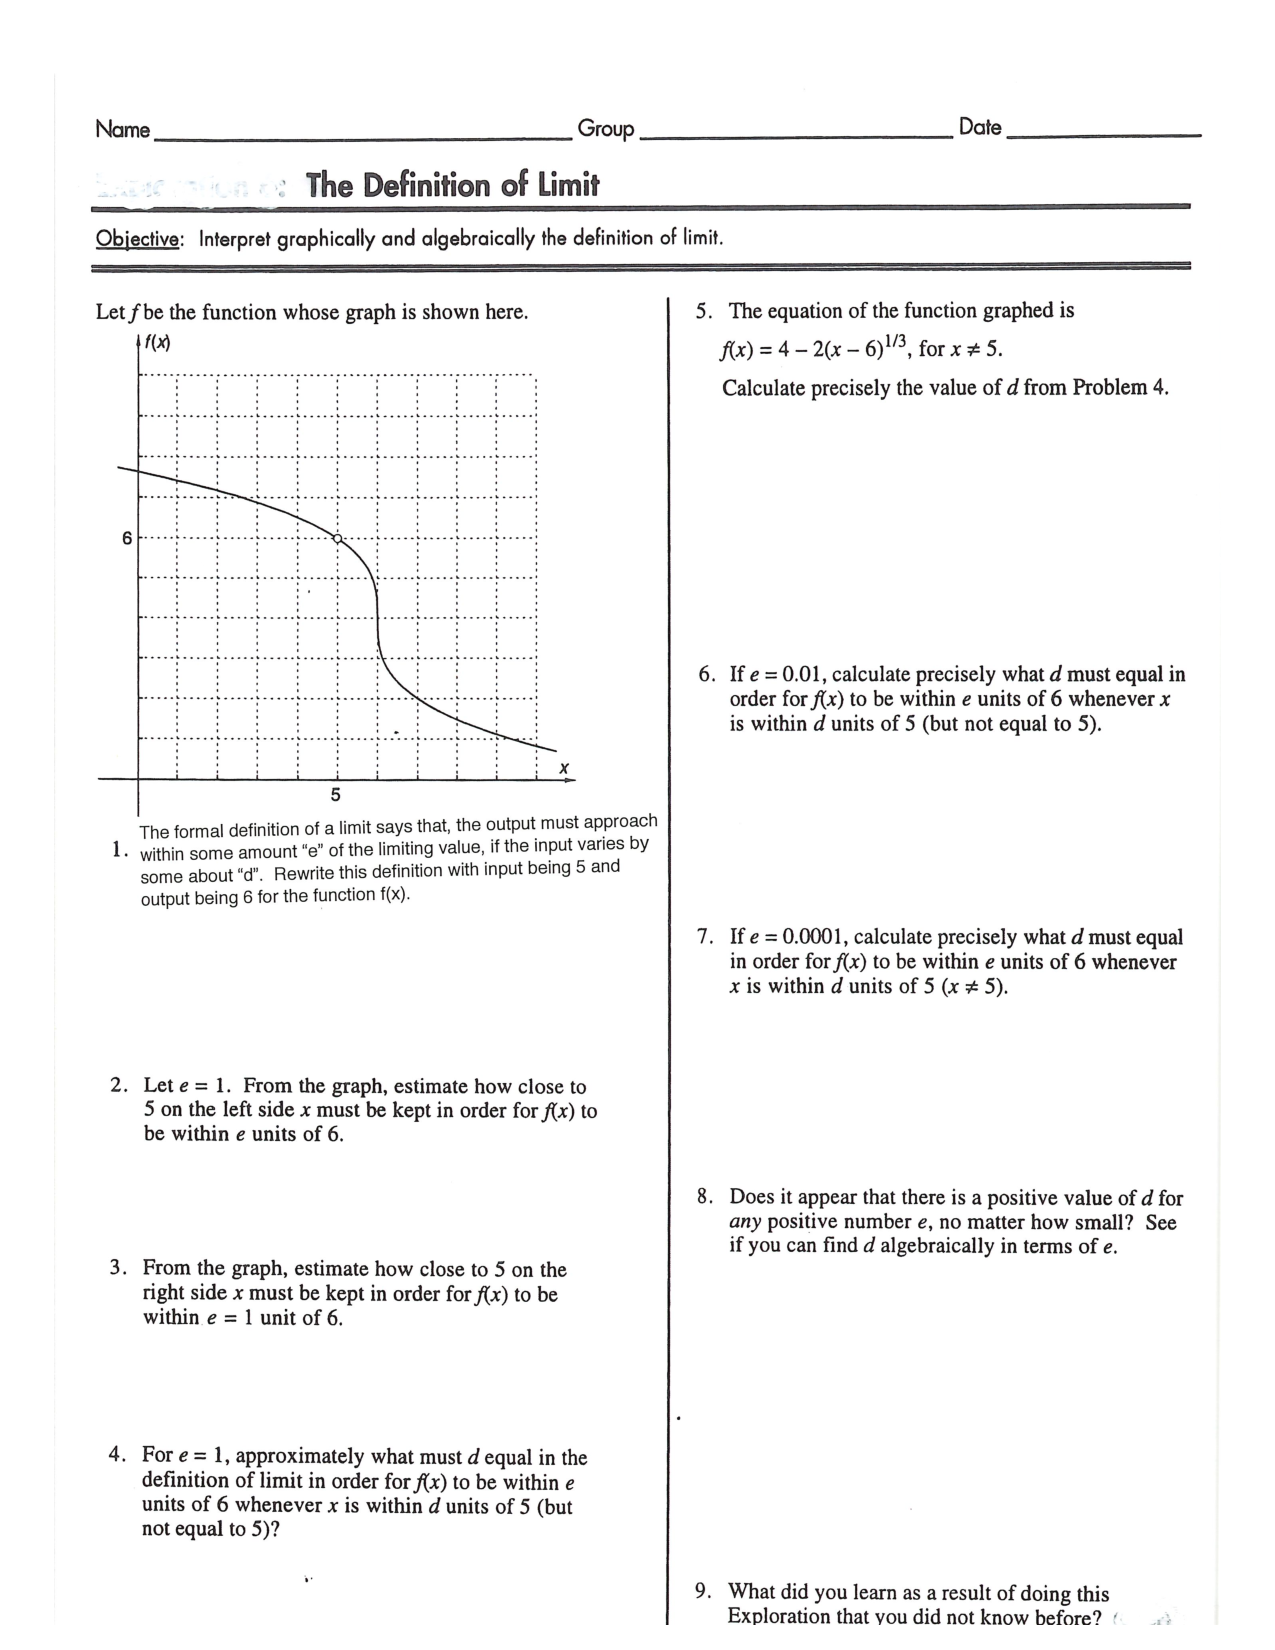
\includegraphics[width=\paperwidth]{\chapdir/0202p.pdf}}
\newpage
%!TEX root =  ../main.tex

\subsection{Epsilon-Delta}

\objective{Use the definition to evaluate limits.}


In the last section, you experiment with finding the values that \emph{would have}
occurred in a series of functions, if there had not been a \textbf{discontinuity} at a given
point.  The value that the function approaches is called a \textbf{limit}.  Because all the
examples to date have been \textbf{removable discontinuities}, it has simply been a matter
of algebra manipulation to produce a \emph{nearly} identical version of the function, but
simply one without the hole.

In the beginning, it was sufficient to define limits as casually as we have done, which is why
2.1 is laid out the way it is.  Later, mathematicians named Cauchy and Weierstrauss created
much more rigorous definitions to meet demand.  Let us built up such rigor.
\marginfig[-1in]{\chapdir/pics/tricky}{The function appears to be a decreasing exponential ... or does it?}

\index{TI-8*!zoom box}
Here is a negative example: $f(x)=\dfrac{|x-3|\cdot1.2^x}{(x-3)\cdot12^x}+2$.  Enter the 
function as $Y_1$ and begin with ZOOM-STANDARD.  You should have a decreasing
exponential function, with a horizontal asymptote at $y=2$.  Now you should become
suspicious.  What did the $x-3$ terms produce?  Is there something going on at $x=3$,
when both terms are 0 and the entire function is $\frac{0}{0}$?  If you consult the
TABLE, you will see there is an ERROR at 3.  Let us investigate.

Practice using the ZOOM-BOX feature, drawing new windows around (3,2) until the 
discontinuity becomes clear.  Here is our window and graph:

insert figure Xmin=2.999 Xmax=3.001 Xscl=5E-4 Ymin=1.9985 Ymax=2.0015 


How can we avoid being fooled like this?  What does it mean to say ``the limit as
$f(x)$ approaches $c$ is $L$''?

\marginfig[-1in]{\chapdir/pics/epsilondelta.png}{Whenever a point $x$ is within $\delta$ units of $c$, $f(x)$ is within $\epsilon$ units of $L$ \cite{epsilondelta}.}



\begin{derivation}{Definition of a Limit}\index{Limit!definition}
$$\lim_{x\rightarrow c} f(x)=L$$


The limit as $x$ approaches $c$ of $f(x)$ is $L$, if and only if
for any $\epsilon>0$ no matter how small, there is a $\delta>0$ such that
$x$ is with $\delta$ units of $c$ but $x\ne c$, that $f(x)$ is with $\epsilon$ units of $L$.
\end{derivation}



In less compact terms, this means for \emph{any} radius $\delta$ around $c$, there is exists
a radius $\epsilon$ around $L$ that $f(x)$ stays with in.  This definition, developed by
Cauchy, is the successor to Leibniz's idea of ``infinitesimals''\footnote{
See \cite{Alexander12}.}.


\subsubsection{Continuity}
It would certainly save a lot of time if we could classify functions by whether they will
ever fail to have a limit or not.  Smooth functions, where every minuscule change in the
input results in a minuscule change in the output are called \textbf{continuous}.  A function
$f(x)$ is continuous at point $a$, if and only if:\index{continuity}
\begin{enumerate}
\item $\displaystyle \lim_{x\rightarrow a} f(x)$ exists,
\item $f(a)$ exist, and
\item $\displaystyle \lim_{x\rightarrow a} f(x) = f(a)$.
\end{enumerate}
A function that is continuous at every point in its domain is said to be a \textbf{continuous
function}.  Continuous functions whose domain is all Real numbers are said to be ``continuous
over the Reals'' or ``continuous for Reals''.


\begin{example}{Discontinuous}
	\exProblem
Is the function $f(x)=\frac{1}{x}$ continuous for Reals?

	\exSolution
No.  In fact, there is \emph{no} $\epsilon$ we could pick that the
output would stay within for any $\delta$ around 0.  The asymptote at $x=0$ shows that the
graph increases \emph{without limit}.


\marginfig[-1.5in]{\chapdir/pics/Function-1_x.png}{Function $y=\frac{1}{x}$\cite{function1x}.}
\end{example}


\begin{example}{Testing the Definition}
	\exProblem
Show that
$$
\lim_{x\rightarrow 1} (5x-3)=2
$$
	\exSolution
According the definition of a limit, we set $c=1$, $f(x)=5x-3$ and let
$L=2$.  To show that $\displaystyle \lim_{x\rightarrow 1}(5x-3)=2$, we need to show that for
any number $\epsilon>0$, there exists a number $\delta>0$ such that for all $x$,

$$
0<|x-1|<\delta \quad \Rightarrow \quad |(5x-3)-2|<\epsilon 
$$

(The symbol $\Rightarrow$ is read ``implies''.)  If we can transform our second equation to 
contain the middle term of the first, we have succeeded:

\marginfig[-1in]{\chapdir/pics/epsilonover5}{$\epsilon-\delta$ around (1,2)}
\begin{align*}
|(5x-3)-2| & < \epsilon \\
|5x-5| & <\epsilon \\
5|x-1| & <\epsilon \\
|x-1| & < \epsilon \div 5\\
\end{align*}
The last line tells us that the original $\epsilon$-inequality will hold is we choose
$\delta < \epsilon \div 5$.


\end{example}
~\vfill
\newpage
\subsection{Exercises}
Made as a Word doc.
~\vfill


%									2 - 3
%\newpage
\invisiblesection{Piecewise}
\subsection{Mind the Gap}
\noindent\makebox[\textwidth]{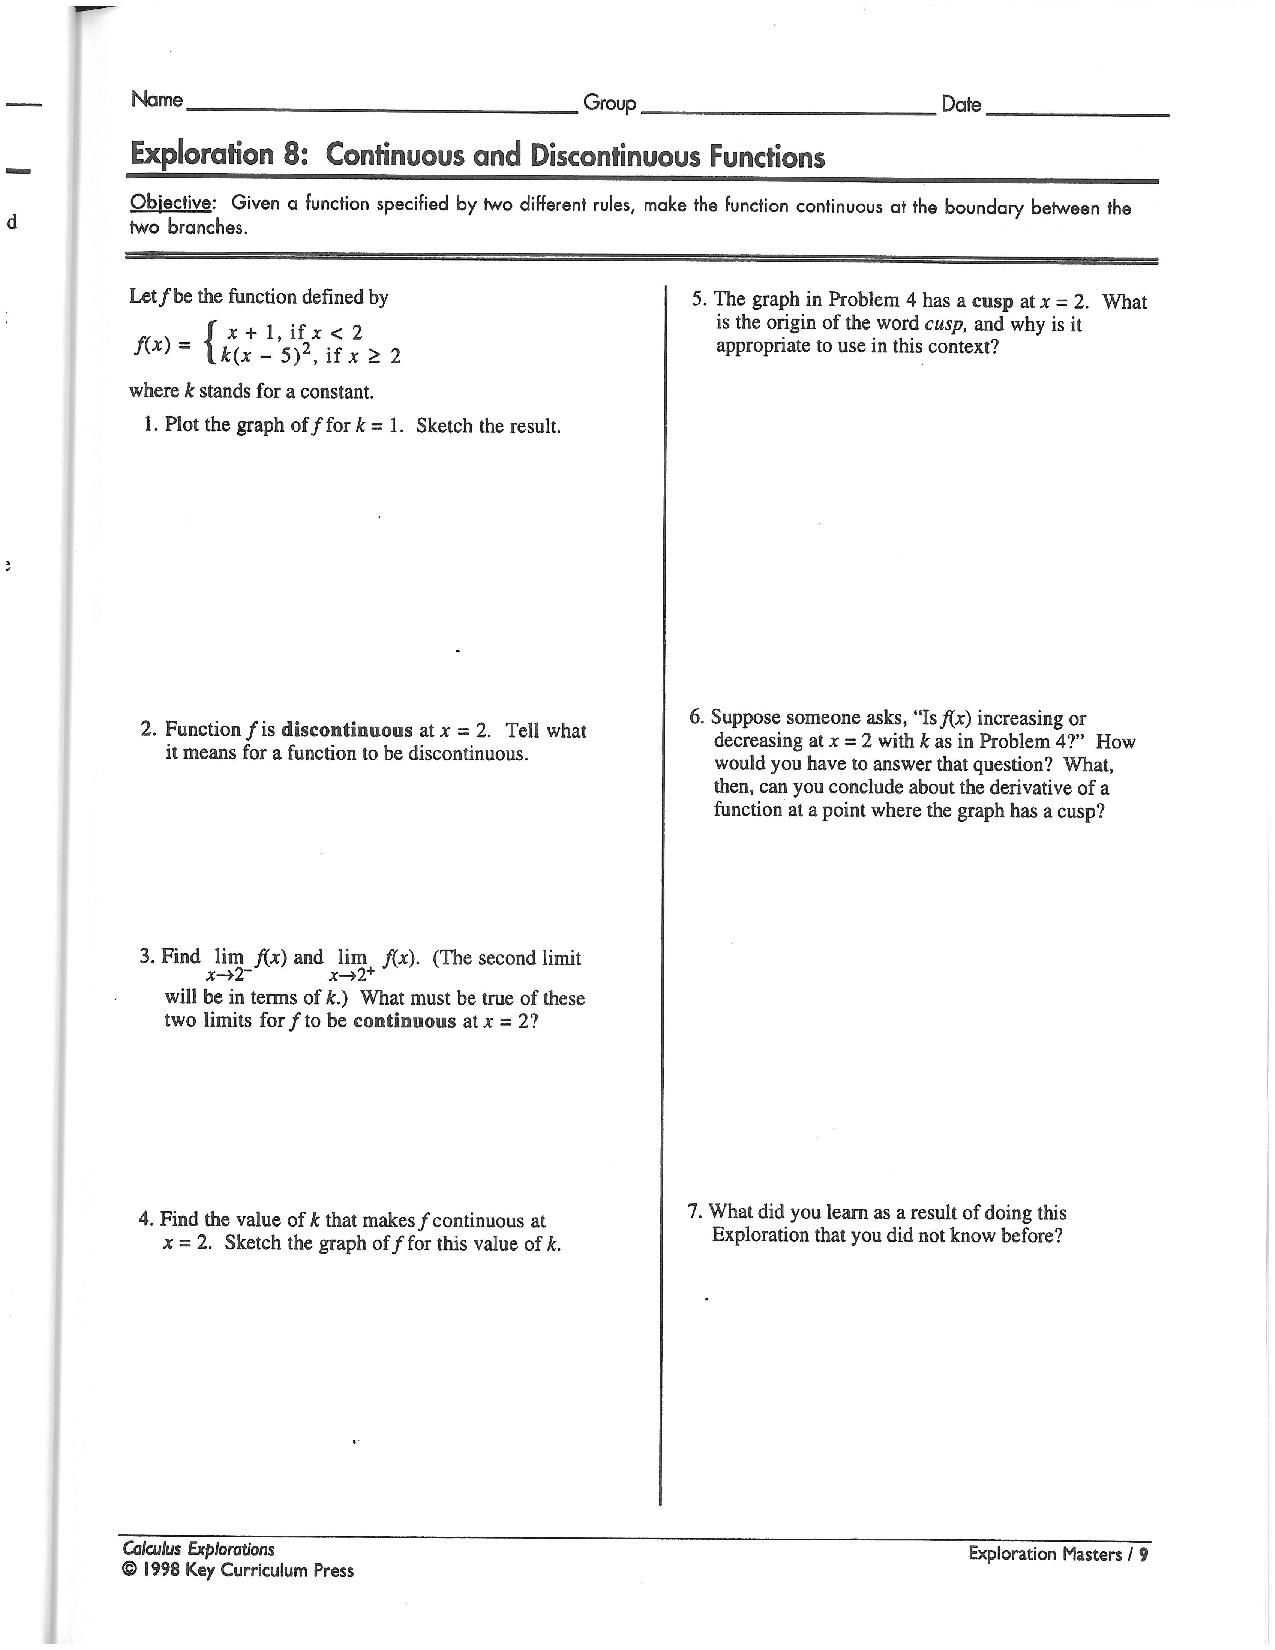
\includegraphics[width=\paperwidth]{\chapdir/0203p.pdf}}
\newpage
%!TEX root =  ../main.tex

\subsection{Definition}

\objective{Interpret piece-wise functions and their limits}


In human observations, there is almost nothing which follows one equation for the 
entirety of its domain.  The only constant in the universe is change!  For example, 
population of the world, the stock market, or even one stock might generally follow one
equation for a significant stretch of time, but not forever.  So it is that most functions are 
defined in pieces, and are therefore called piece-wise functions.

For example, the absolute value function which you have been using for some time now is
actually a piecewise function.\index{Absolute Value!piece-wise}

We should formally define the nomenclature of a ``sided'' limit:

\begin{derivation}{Right-sided limit}\index{limit!right-sided}
``The limit as $x$ approaches $c$ from the right is $L$'' is true if and only if for every $\epsilon > 0$, there exists a $\delta > 0$ such that
$|f(x)-L|<\epsilon$ whenever $0<x-c<\delta$.

$$\lim_{x \to c^+}f(x) = L$$
\end{derivation}


\begin{derivation}{Left-sided limit}\index{limit!left-sided}
Similarly, ``The limit as $x$ approaches $c$ from the left is $L$'' is true if and only if for every $\epsilon > 0$, there exists a $\delta > 0$ such that
$|f(x)-L|<\epsilon$ whenever $0<c-x<\delta$.

$$\lim_{x \to c^-}f(x) = L$$
\end{derivation}


\personfeature[-3in]{George_Boole_color}{George
    Boole}{1815-1864, French}{was an English mathematician
    who said, ``No general method for the solution of questions 
    in the theory of probabilities can be established which does 
    not explicitly recognise, not only the special numerical bases 
    of the science, but also those universal laws of thought which 
    are the basis of all reasoning, and which, whatever they 
    may be as to their essence, are at least mathematical as to their form.''
    \href{https://en.wikipedia.org/wiki/George_Boole}{(Wikipedia)}}

\subsubsection{Boolean Variables}\index{booleans}
Perhaps surprisingly, your TI-8* can graph piece-wise functions.  We will start with a simple
piecewise-function :

$$
f(x)=
\begin{cases}
x, x<1\\
x^2,x\ge 1
\end{cases}
$$

\index{TI-8*!piece-wise}


If we wanted to graph the sections separately, we could make $Y_1=(X^2)/(X\ge{}1)$ and
$Y_2=(X)/(X<1)$.  (The equality and inequality signs are under 2ND-MATH --- TEST.)  This will 
allow you to make the different sections different colors or different shading, but that might be
what you want.  To graph everything in $Y_1$, use $(X^2)*(X\ge{}1)+(X)*(X<1)$.



\subsection{Other Discontinuities}
\reminder{\lefthand}{The different TI-8* behave differently around holes.  Newer calculators will attempt to make a hole apparent, while older models do not show it.

Only the new models draw points visibly, but even then they are very small.  We recommend
against even trying to represent them in the TI-8*.}


All together, there are five kinds of discontinuities.  We are only responsible to rigorously prove
instanes of the first two and the last:

\subsubsection{Removable}
Here the limit exist.  The graph has a hole in it, which may or may not be defined as a point somewhere unexpected.
\subsubsection{Jump}
The limits does not exist.  The graph is not continuous, but ``leaps'' from one output to another without passing in between, at one or more points.
\subsubsection{Infinite} 
The limit may or may not exist.  The function itself goes up and/or down without limit.  The most common example is a vertical asymptote.
\subsubsection{Oscillating} 
The limit does not exist.  The graph varies between outputs in way that never resolves.
\subsubsection{Domain} 
The limits does not exist because on one side, the function ceases to exist.



%\newpage
\subsection{Exercises}
\noindent\makebox[\textwidth]{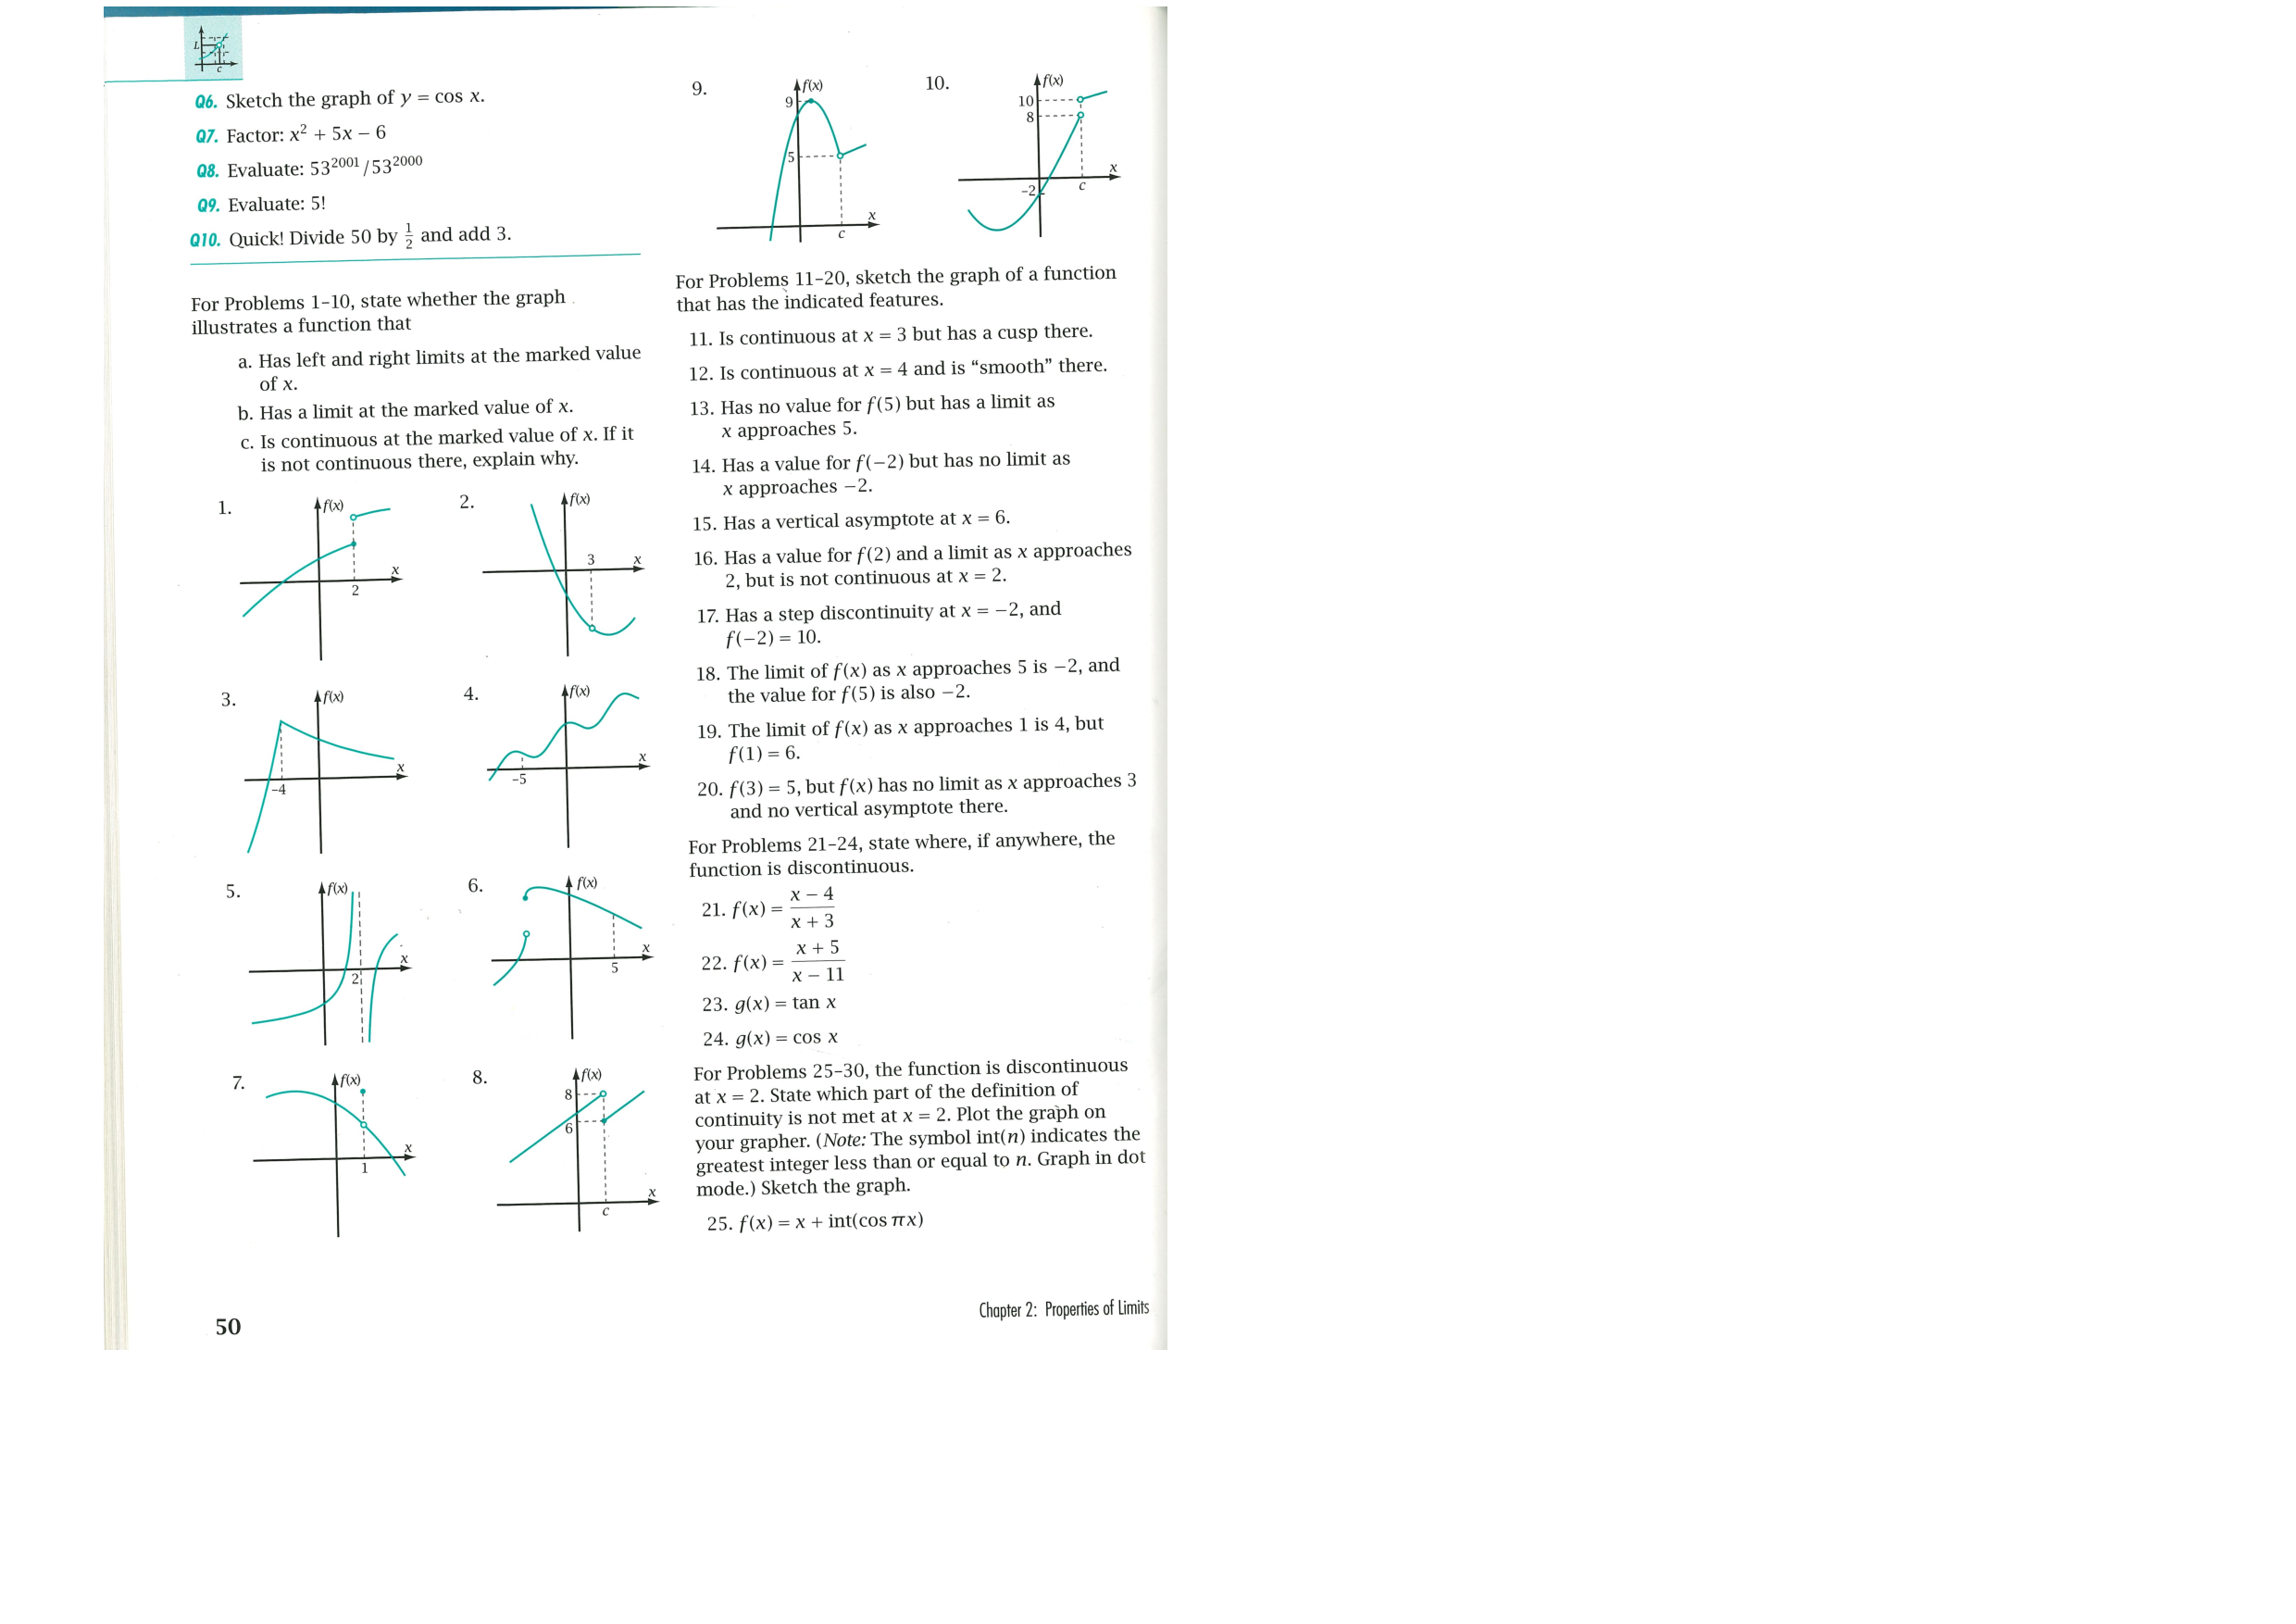
\includegraphics[width=\paperwidth]{\chapdir/0203xA.pdf}}
\newpage
\noindent\makebox[\textwidth]{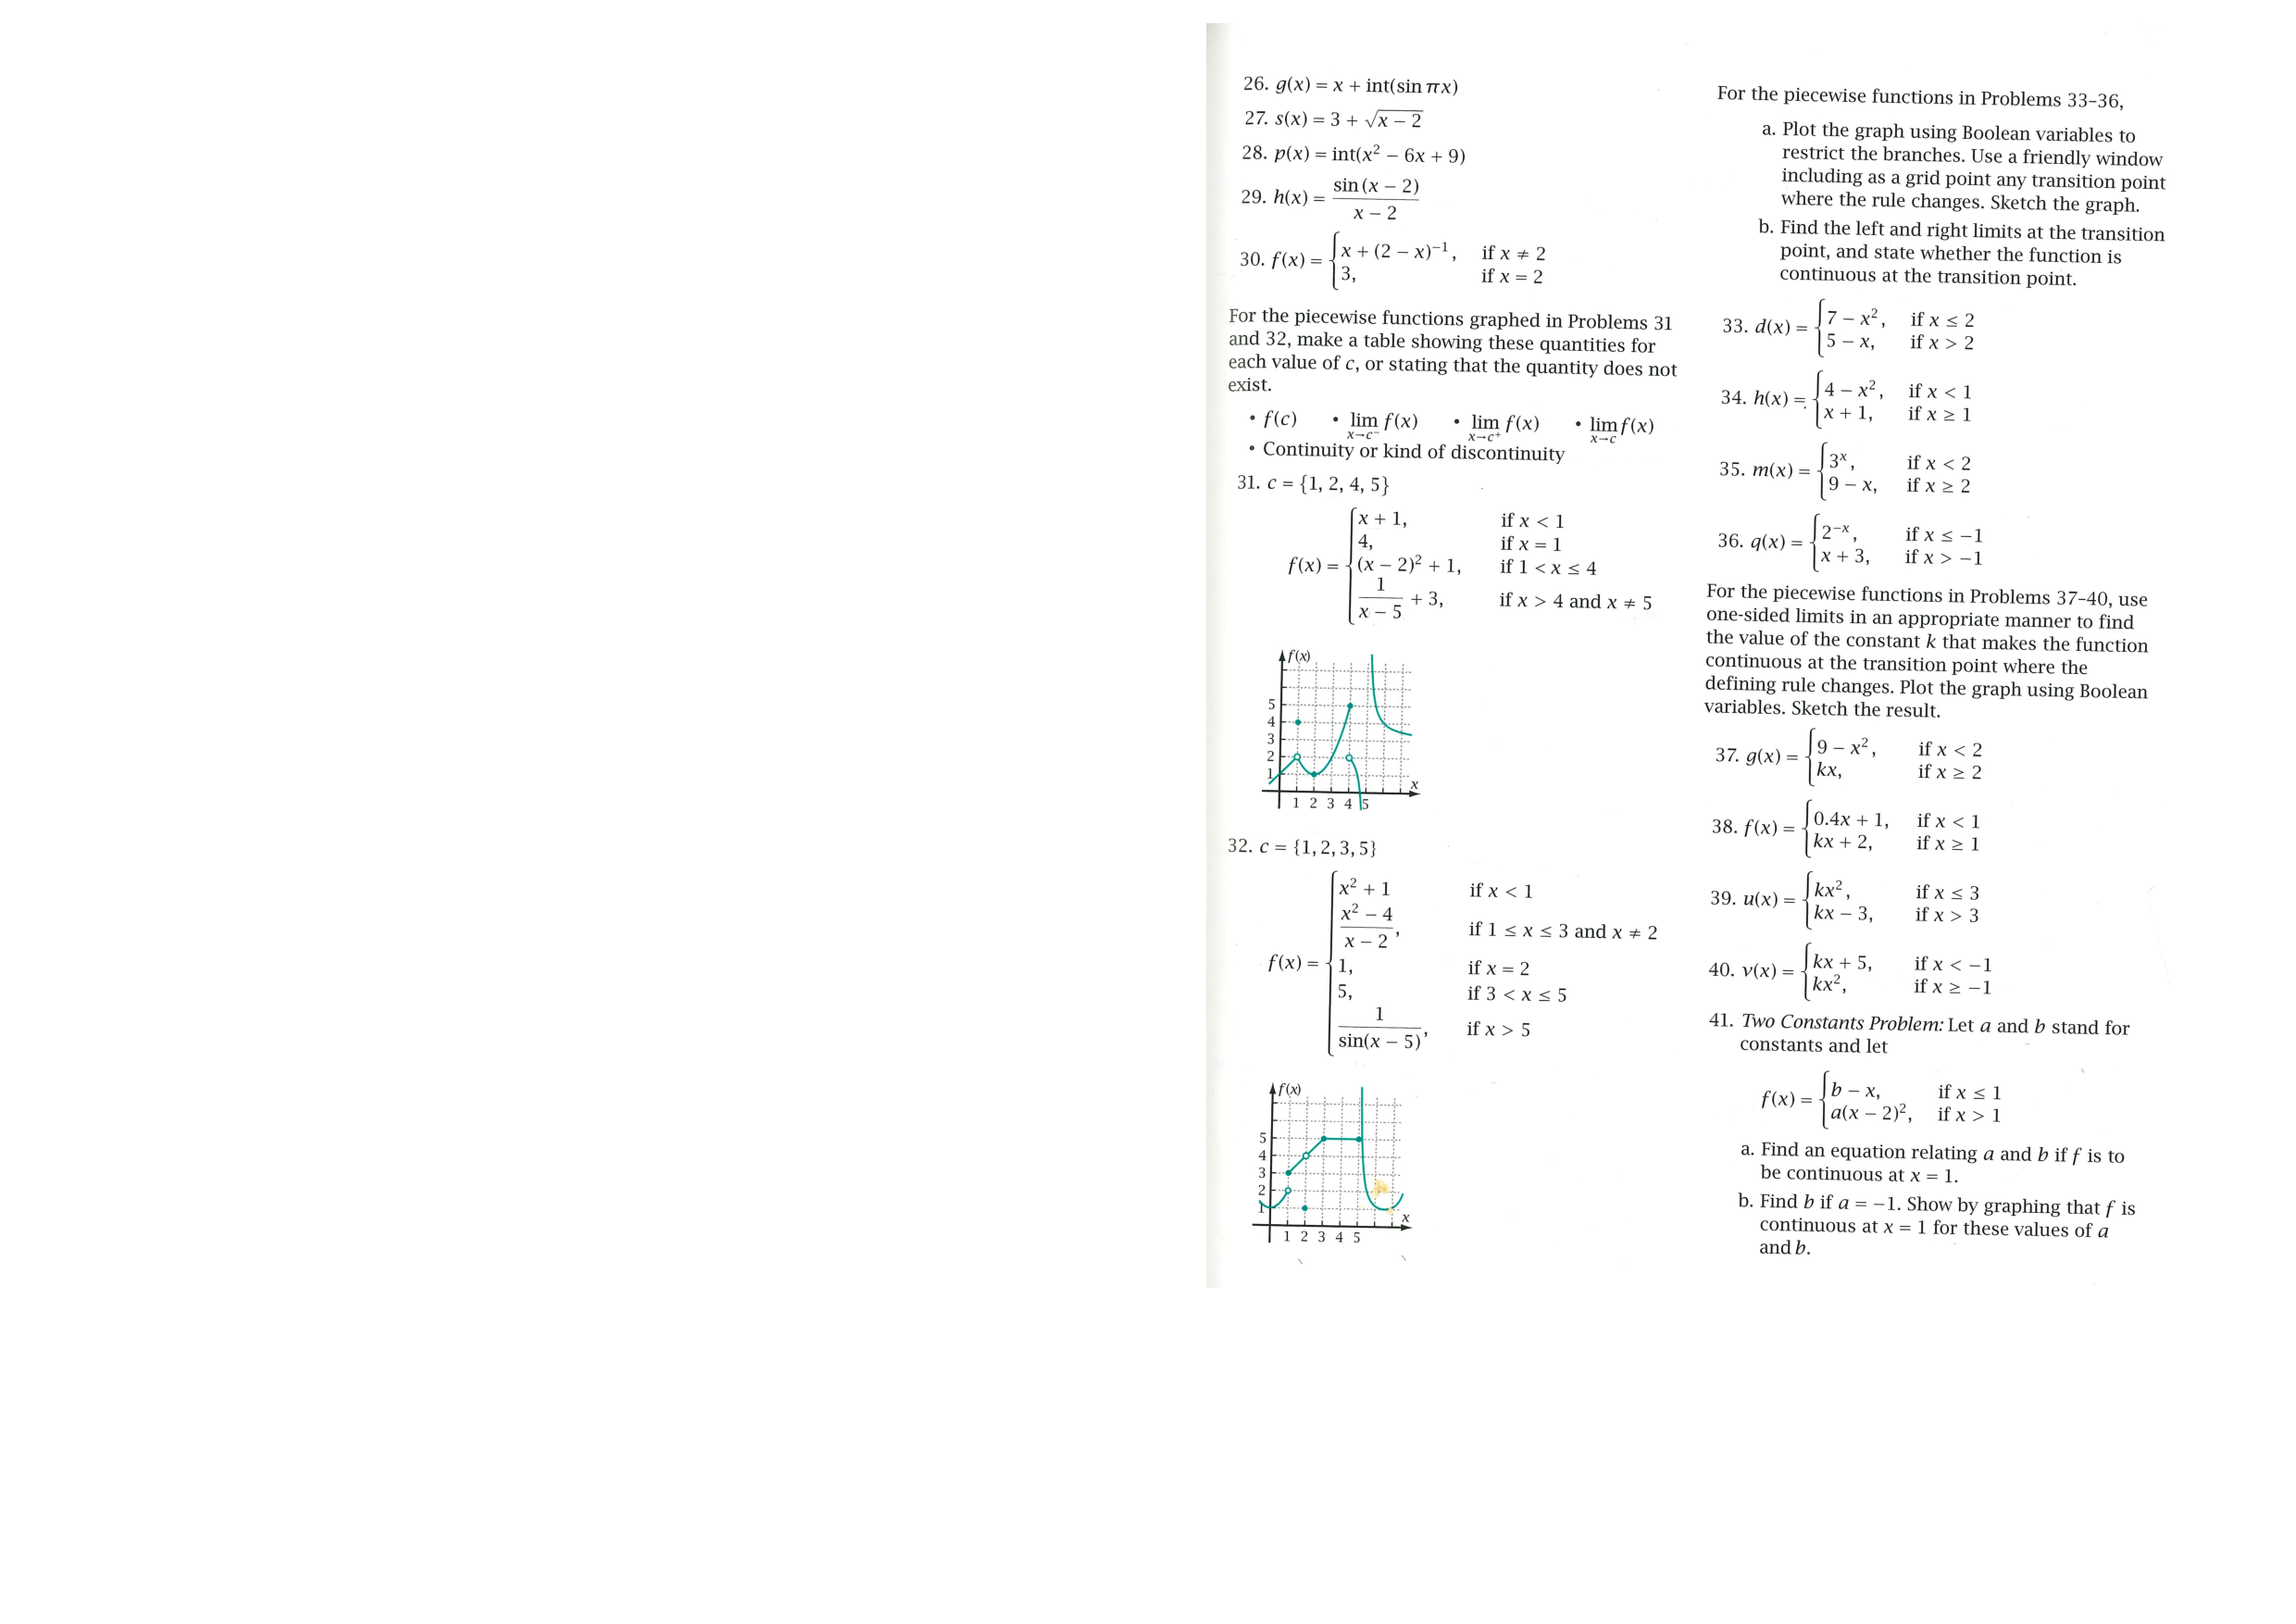
\includegraphics[width=\paperwidth]{\chapdir/0203xB.pdf}}
\noindent\makebox[\textwidth]{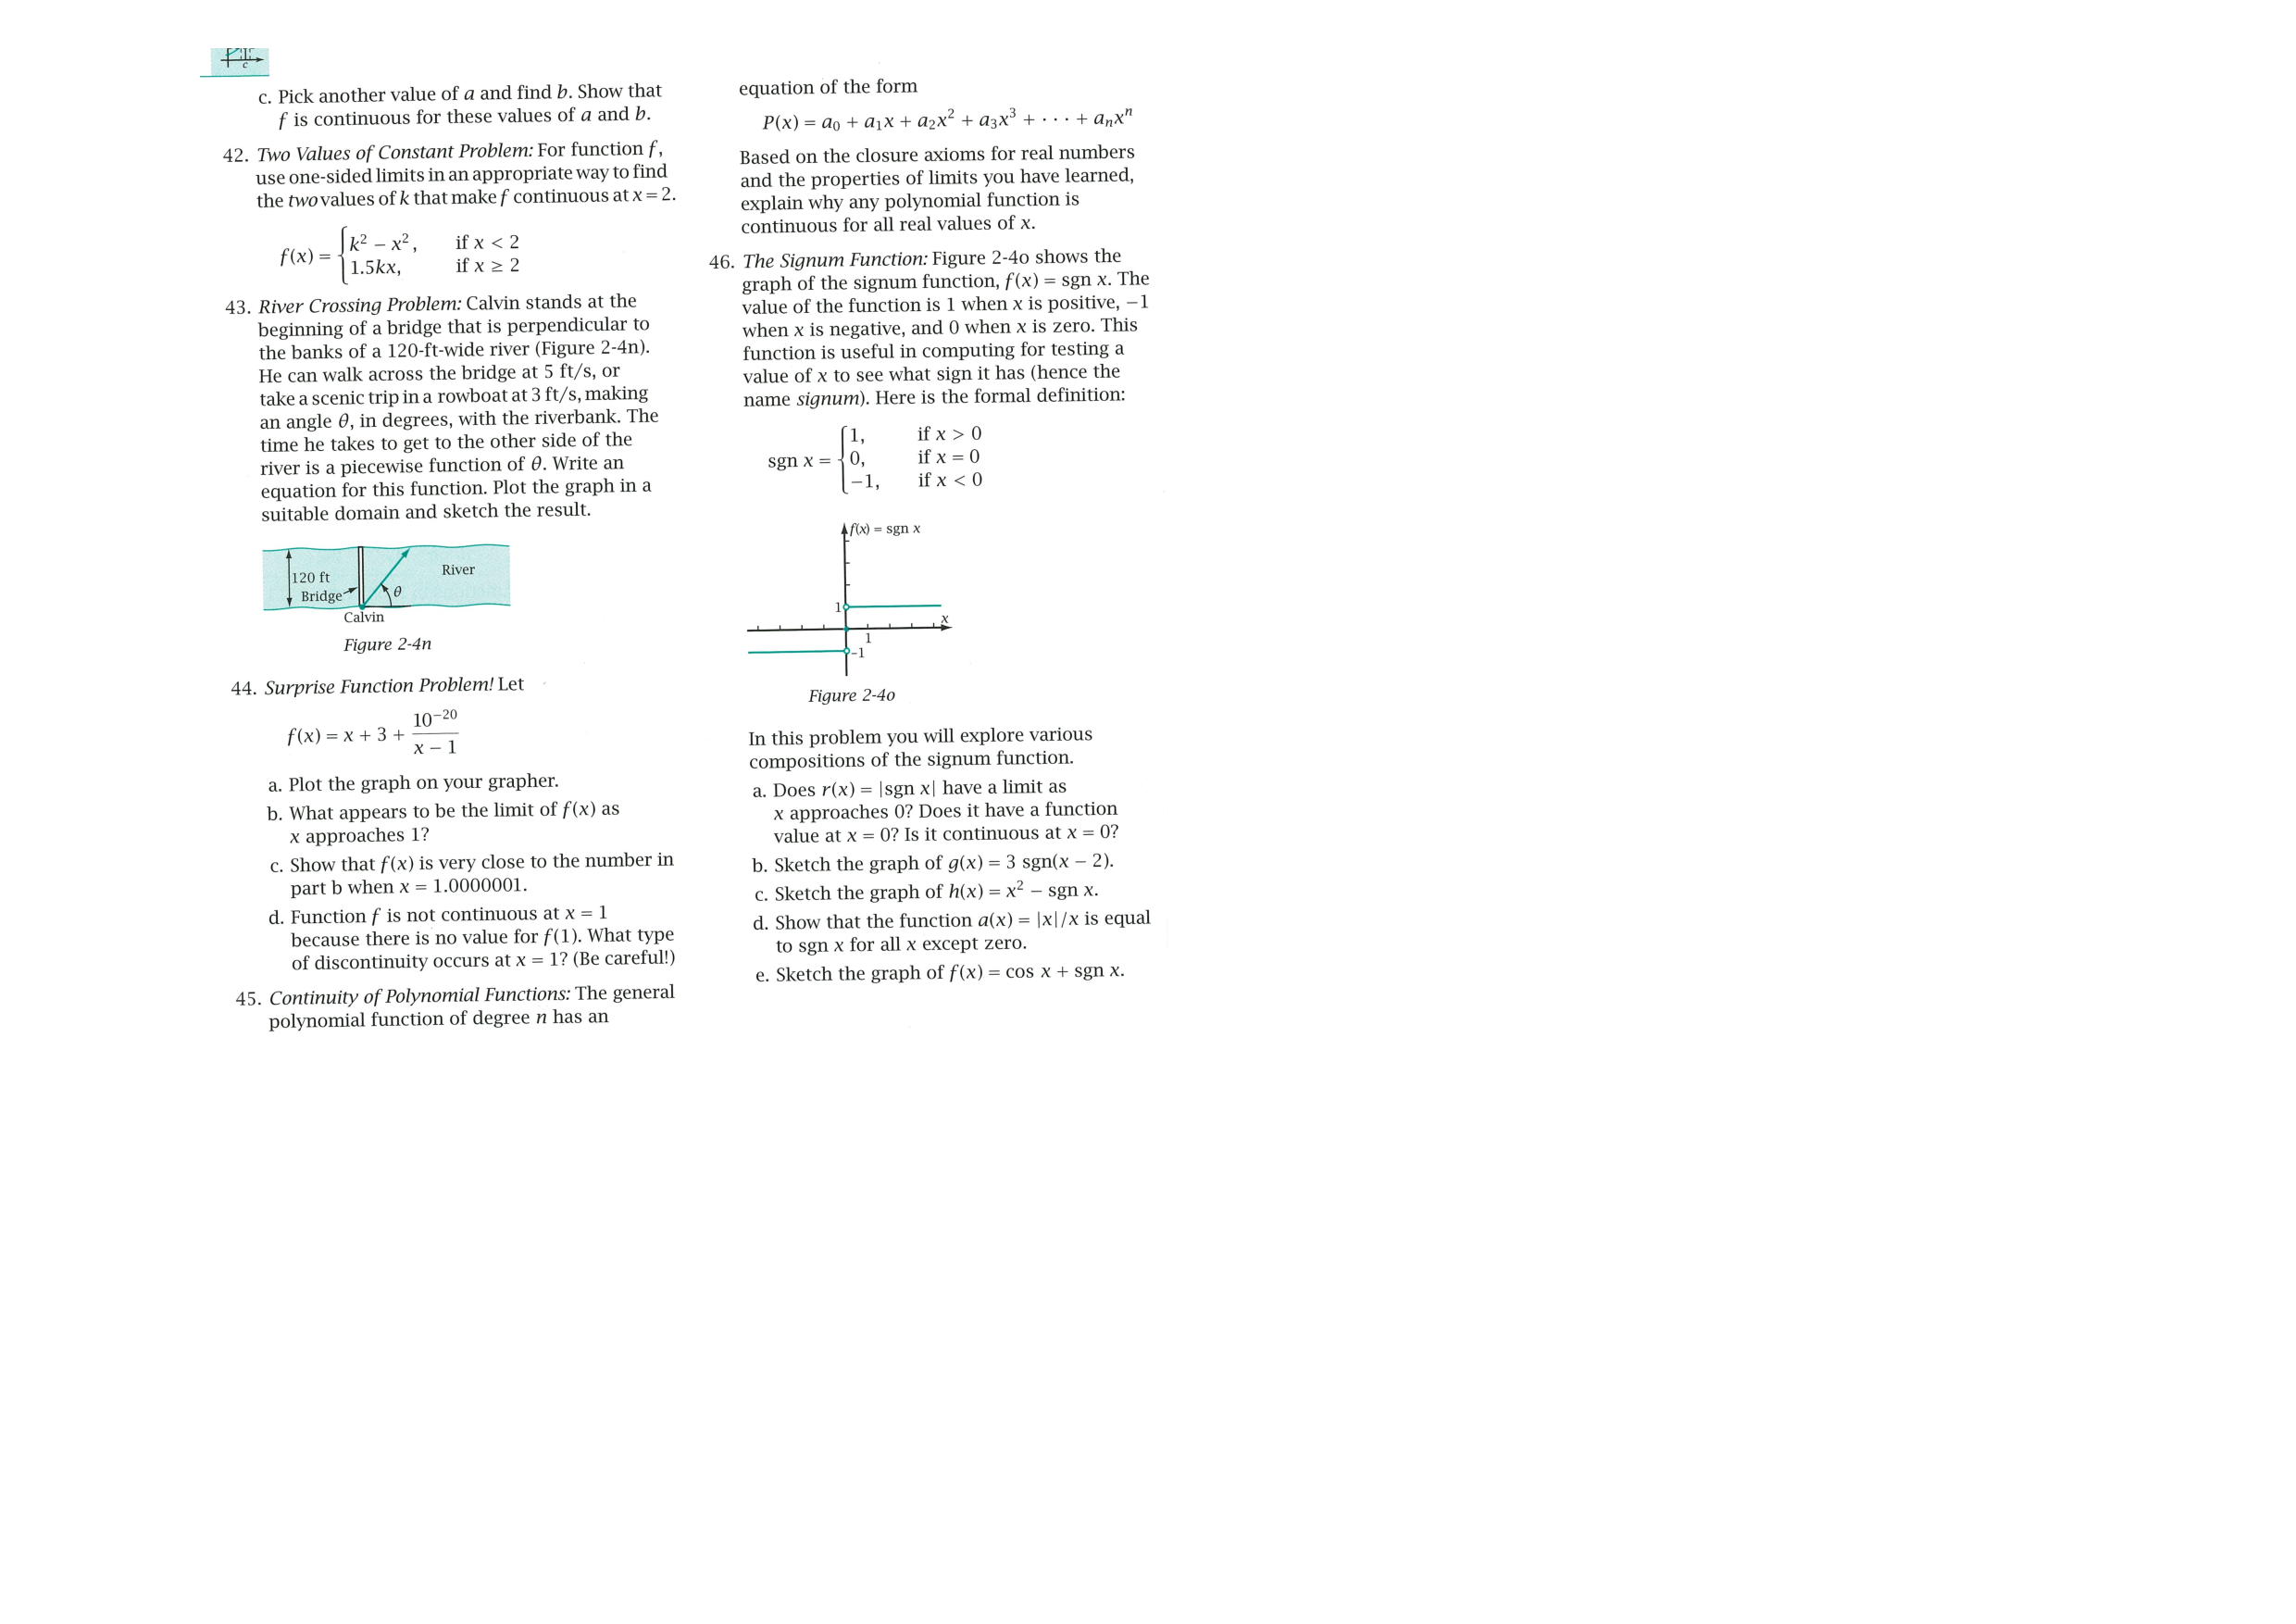
\includegraphics[width=\paperwidth]{\chapdir/0203xC.pdf}}




%									2 - 4
\invisiblesection{Infinite}
\subsection{Are We There Yet?}
\noindent\makebox[\textwidth]{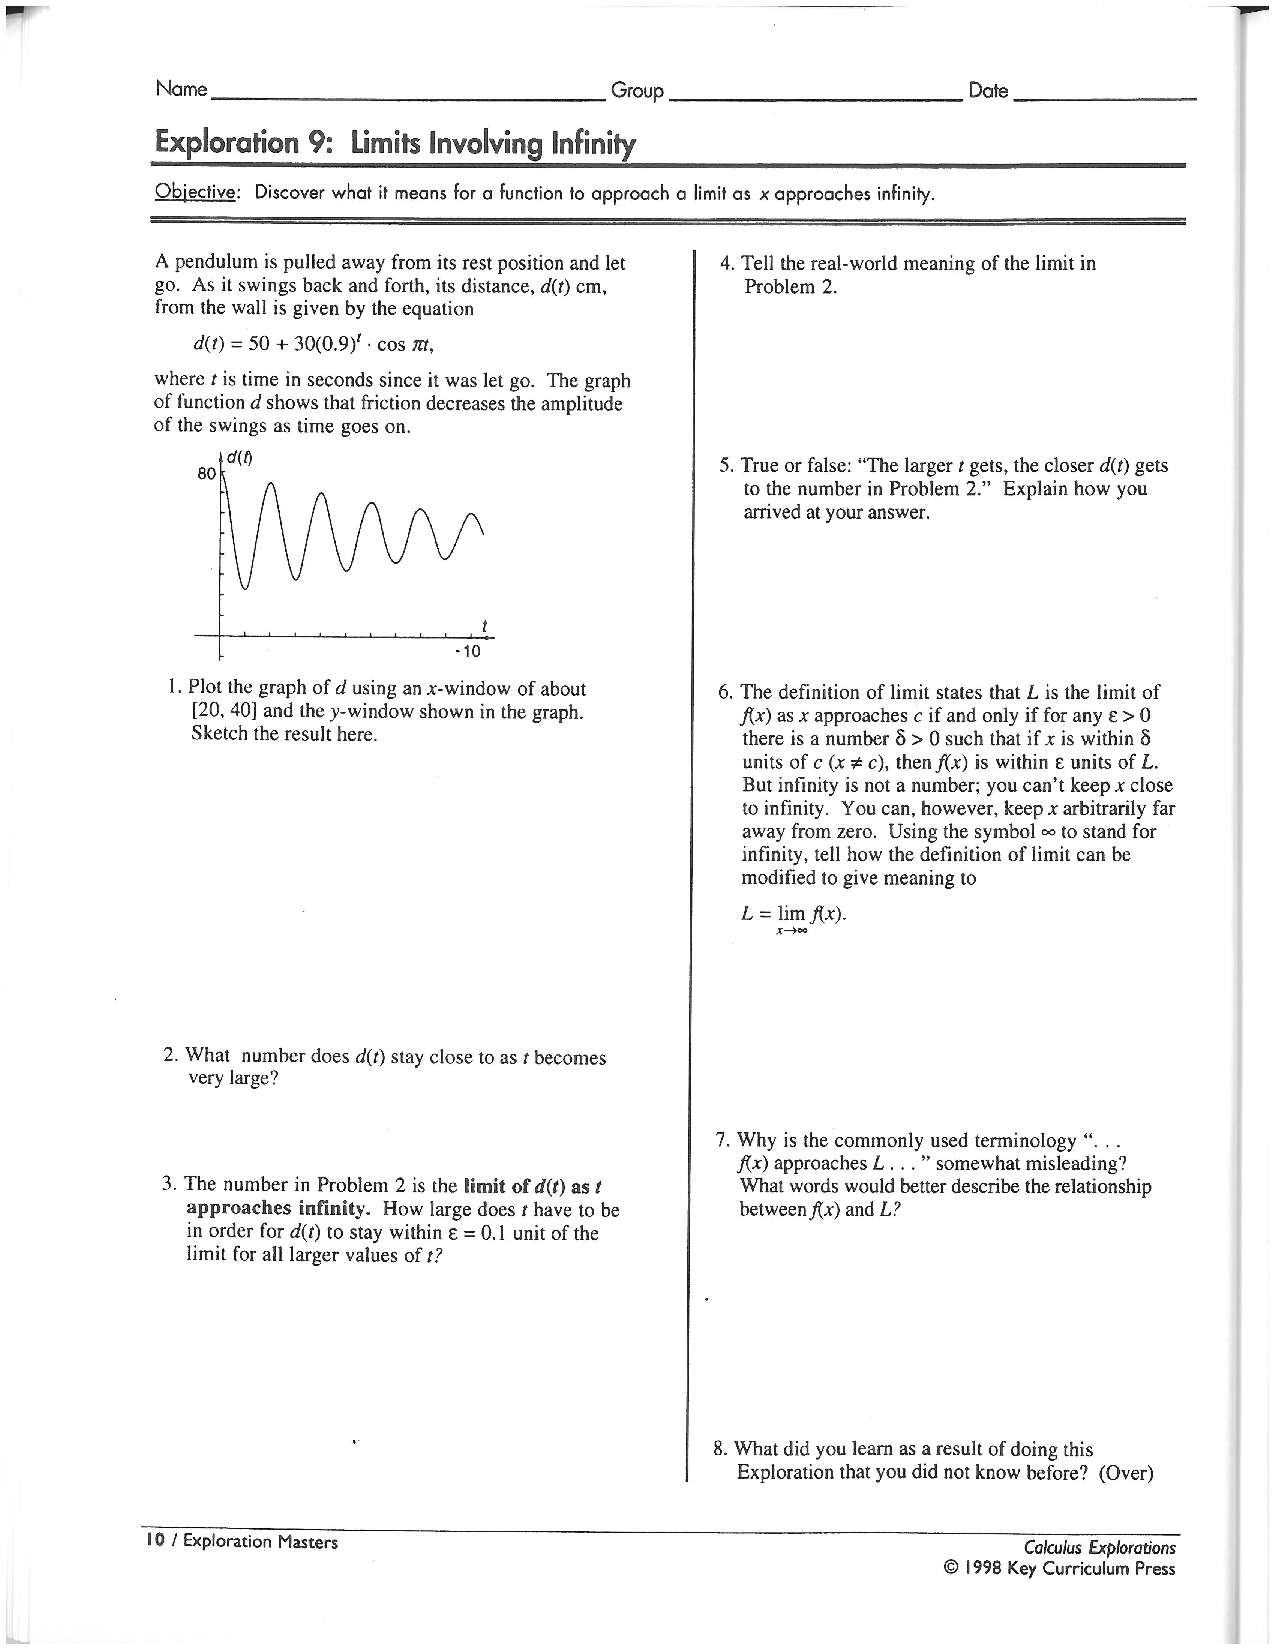
\includegraphics[width=\paperwidth]{\chapdir/0204p.pdf}}
%!TEX root =  ../main.tex

\subsection{At Infinities}

\objective{Determine when a limit does and does not exist, or is infinite.}

Because limits are asking questions that need not have simple number inputs and
need not have simple number outputs, we can evaluate limits involving infinities.
``Infinity'' simply means ``without end''.  Asking what a function approaches as
$x$ approaches infinity, graphically means ``what value is the output tending
towards as the input grows without bound?''.  Negative infinity is a term describing
the leftward trend of function.


\begin{derivation}{Limit at Infinity}
For $f(x)$ a real function, the limit of $f$ as $x$ approaches infinity is L, 
means that for all  $\varepsilon >0$, there exists $c$ such 
that $|f(x) - L| < \varepsilon \text{whenever} x > c$. \footnote{$\forall \varepsilon > 
0 \; \exists c \; \forall x > c :\; |f(x) - L| < \varepsilon$}

$$\lim _{x\to \infty }f(x)=L$$

\end{derivation}


The same applies at negative infinity:


\begin{derivation}{Limit at Negative Infinity}\index{limit!at infinities}
For $f(x)$ a real function, the limit of $f$ as $x$ approaches negative infinity is L, 
means that for all $\varepsilon >0$ there exists $c$ such that 
$ |f(x) - L| < \varepsilon \text{whenever} x < c$.  \footnote{$\forall \varepsilon > 
0 \; \exists c \; \forall x < c :\; |f(x) - L| < \varepsilon$}


$$ \lim_{x \to -\infty}f(x) = L$$

\end{derivation}


\begin{example}
	\exProblem
Evaluate $\displaystyle \lim_{x \to -\infty}2^x$
	\exSolution
We can observe the graph or compute numerically that $2^x$ is getting closer
and closer to 0 as we move leftward.  We can get arbitrarily close to 0 by picking
whatever large, negative exponent we wish.  Hence, the answer is 0
\end{example}




\subsection{Infinite Forms}
Not only can we ``plug in'' infinities in limits problems, but we can also get
$\pm\infty$ as an answer.  Recall, however, that the left and right sided limits
must agree for the limit to exist.  Hence, we can say that the limit as $x$ 
approaches 0 of $x^{-2}$ is infinity, while the same limit taken on $\frac{1}{x}$
does not exist.


the limit of f as x approaches a is infinity, denoted

$$\lim_{x \to a} f(x) = \infty$$
means that for all $\varepsilon >0 \text{there exists}  \delta >0 \text{such that}  f(x) > \varepsilon \text{whenever}  |x - a| < \delta$.

These ideas can be combined in a natural way to produce definitions for different combinations, such as

$$f(x)=  \lim_{x \to \infty} f(x) = \infty, \lim_{x \to a^+}f(x) = -\infty$$.
For example:

$$ \lim_{x \to 0^+} \ln x = -\infty$$

%\newpage
\subsection{Exercises}
\noindent\makebox[\textwidth]{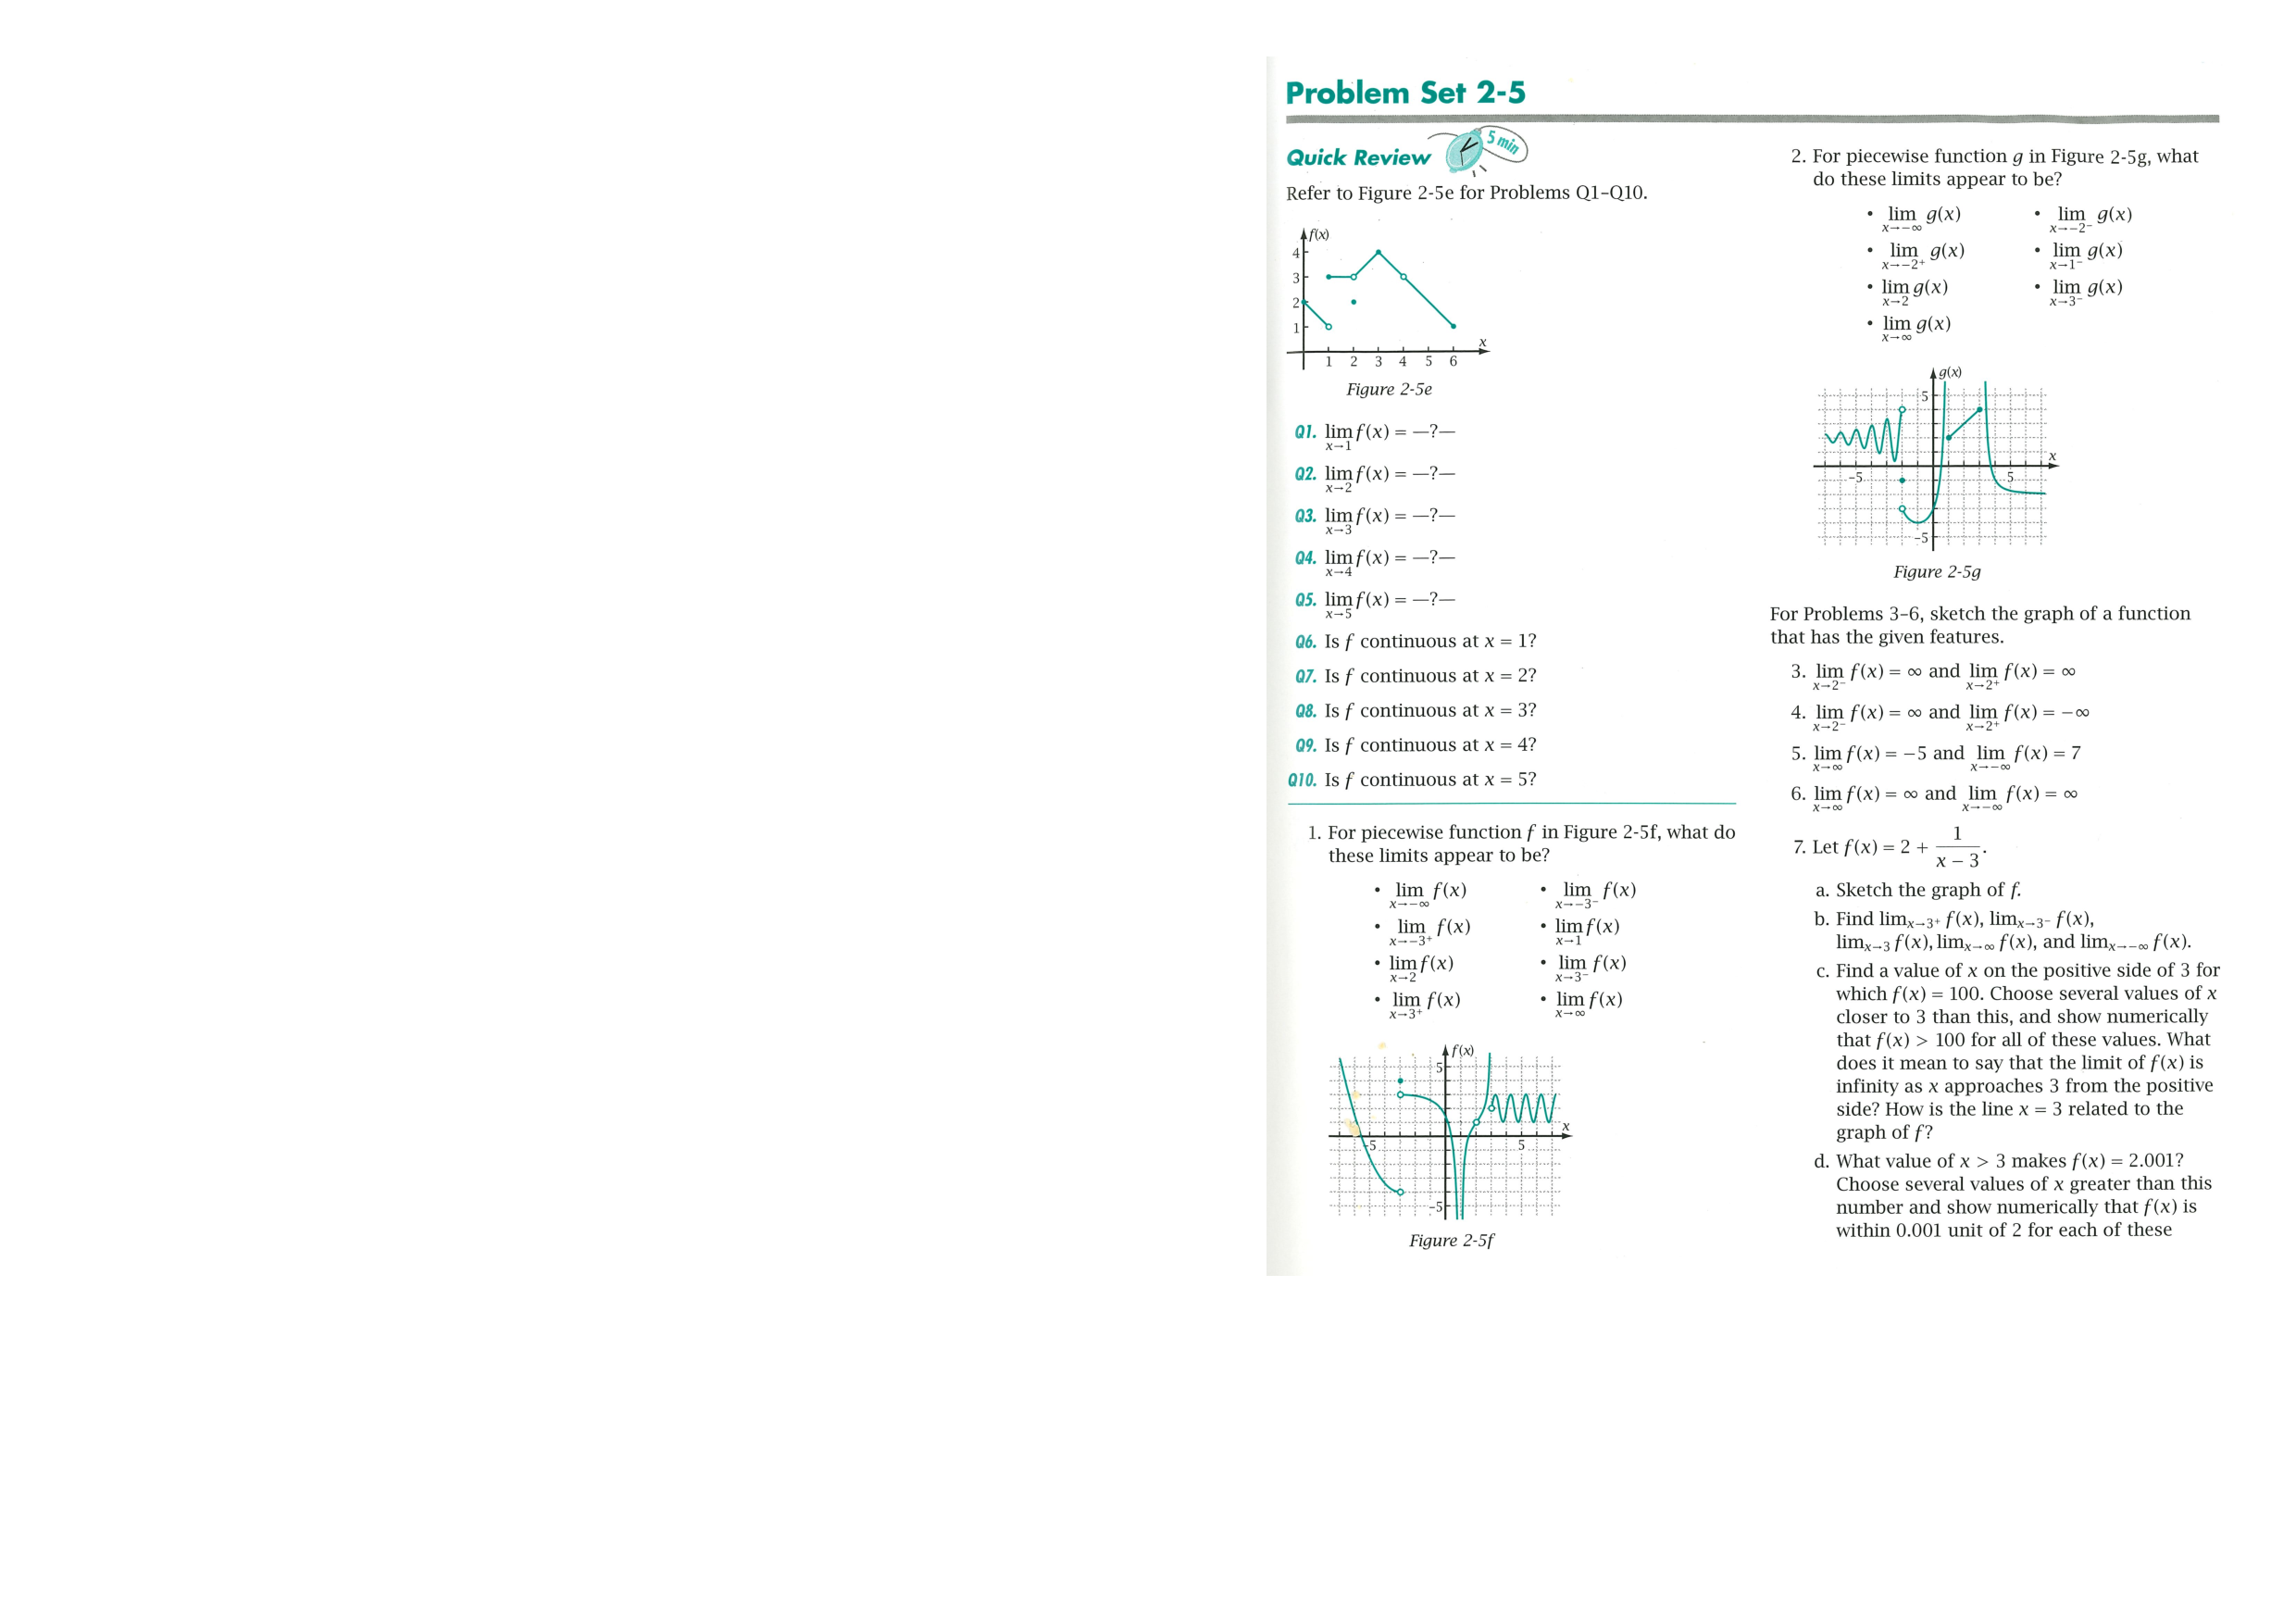
\includegraphics[width=\paperwidth]{\chapdir/0204xA.pdf}}
\newpage
\noindent\makebox[\textwidth]{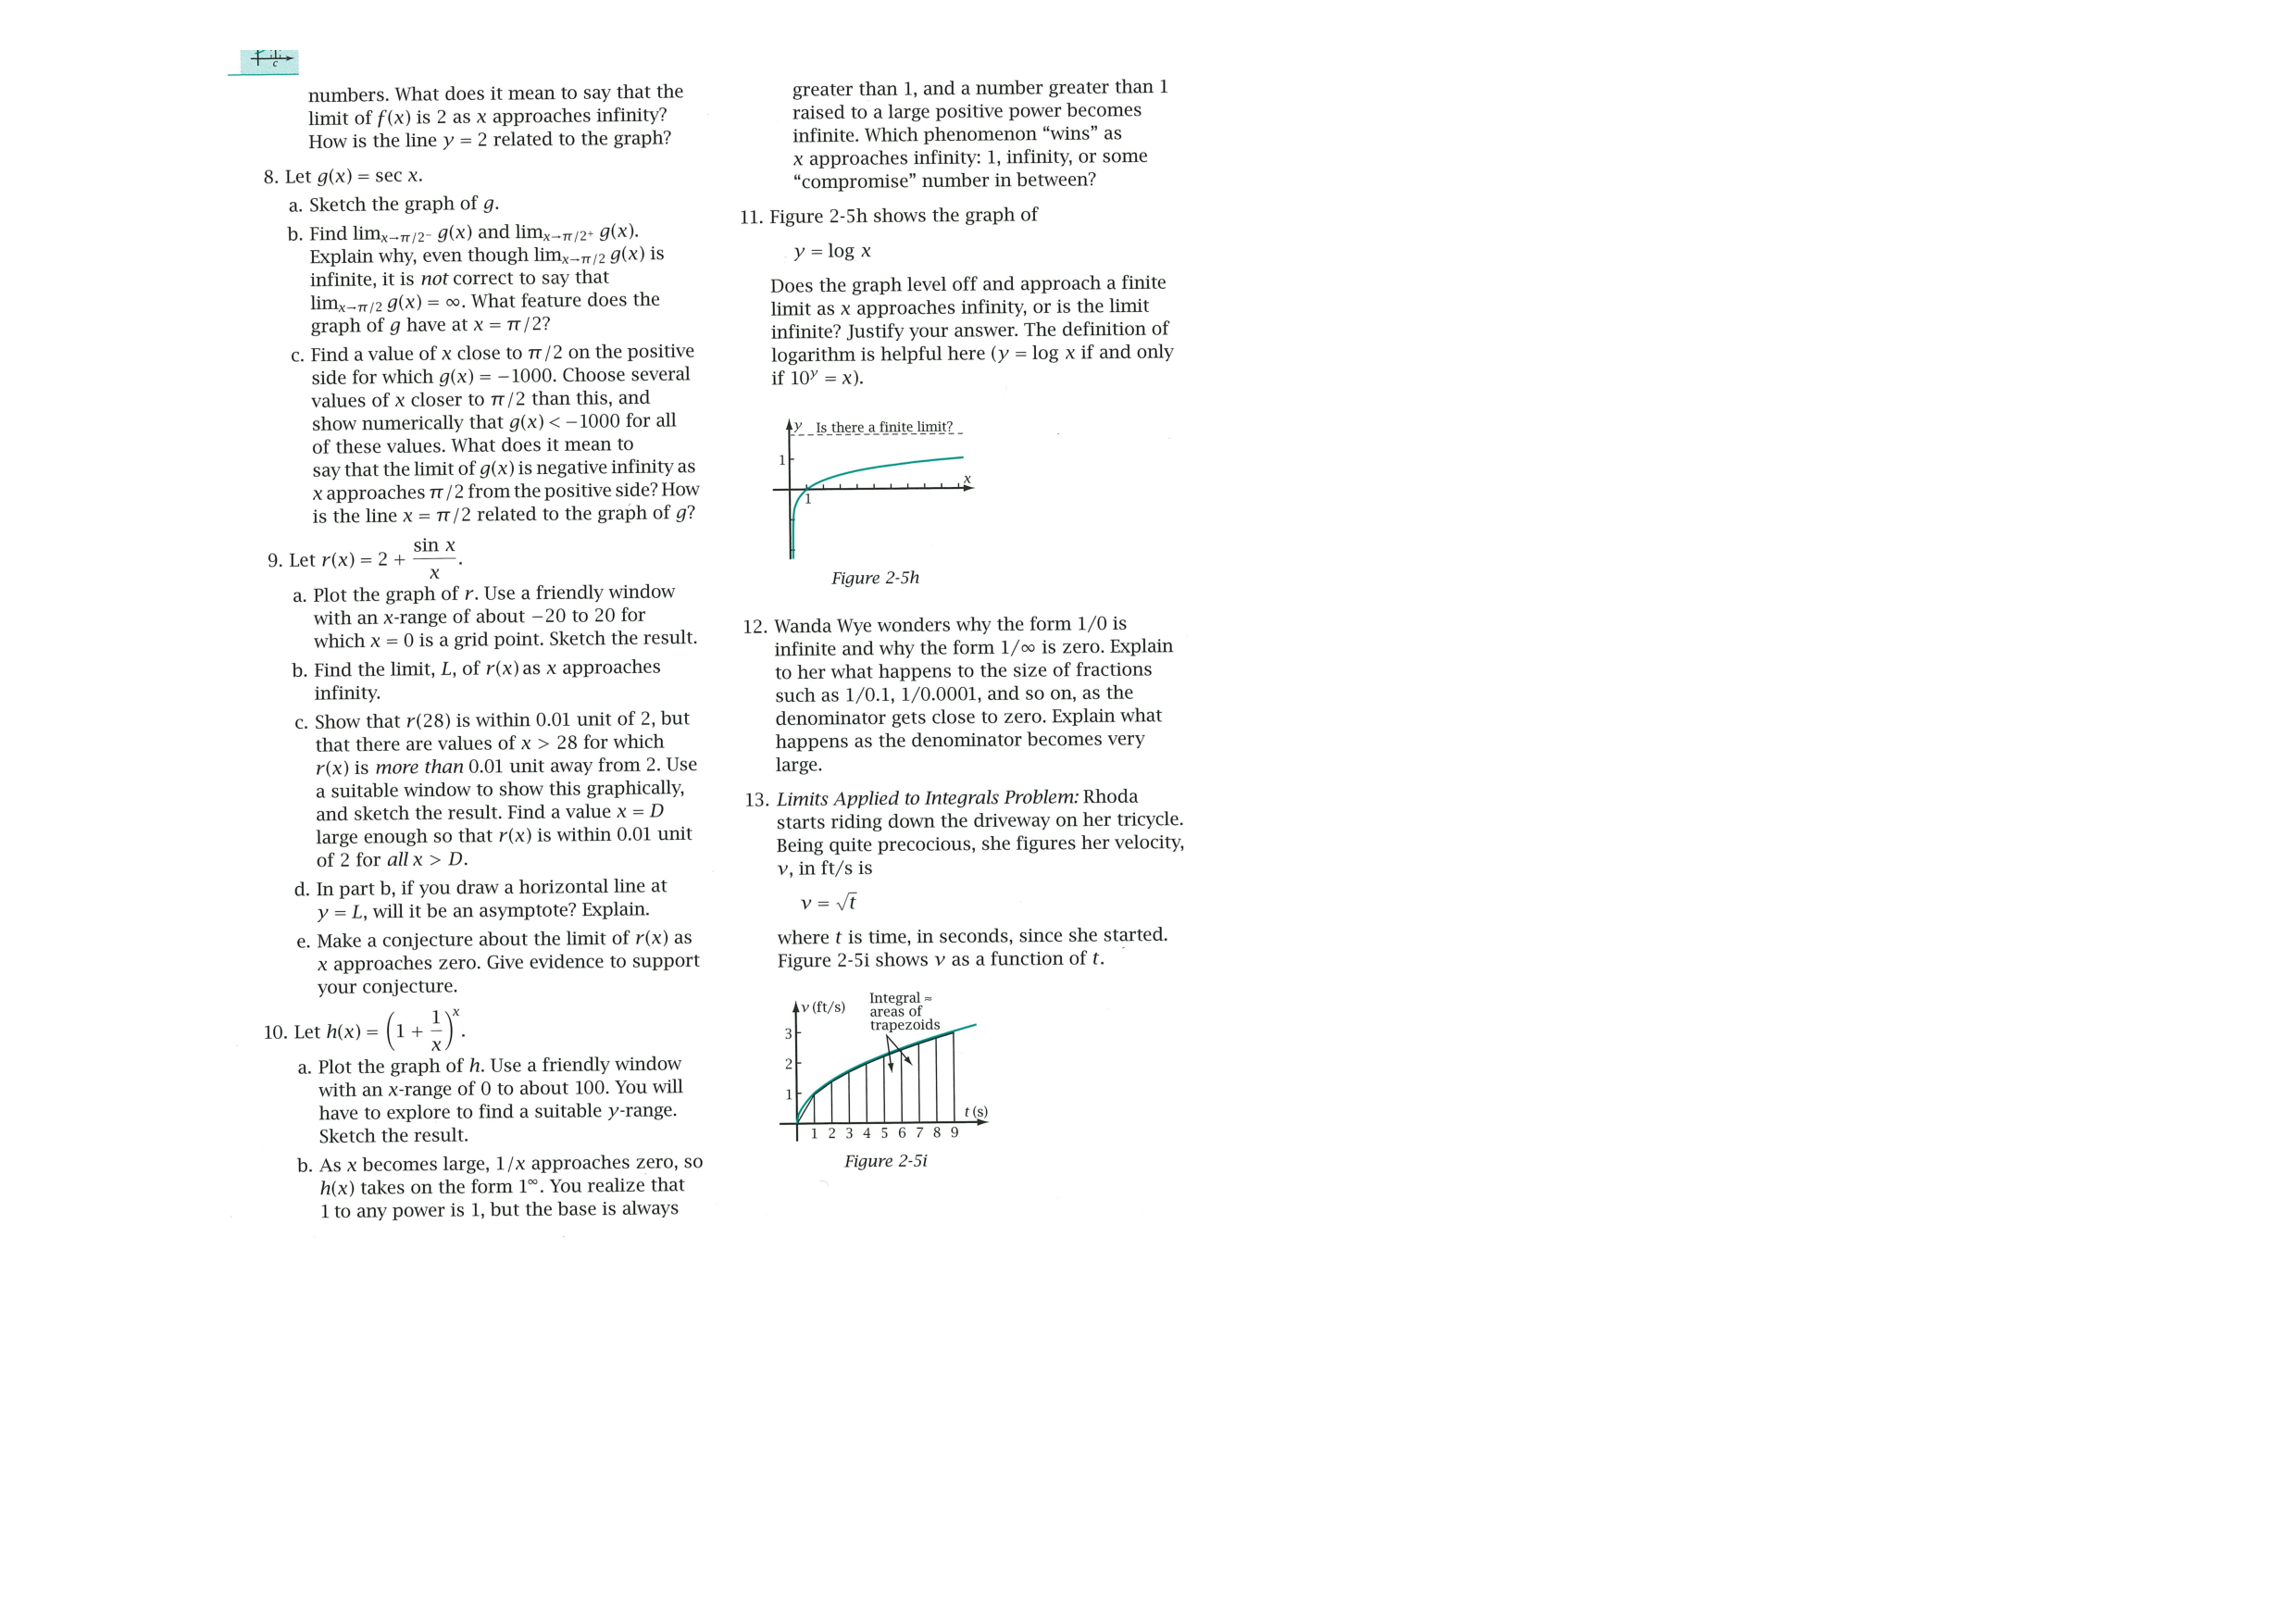
\includegraphics[width=\paperwidth]{\chapdir/0204xB.pdf}}
\noindent\makebox[\textwidth]{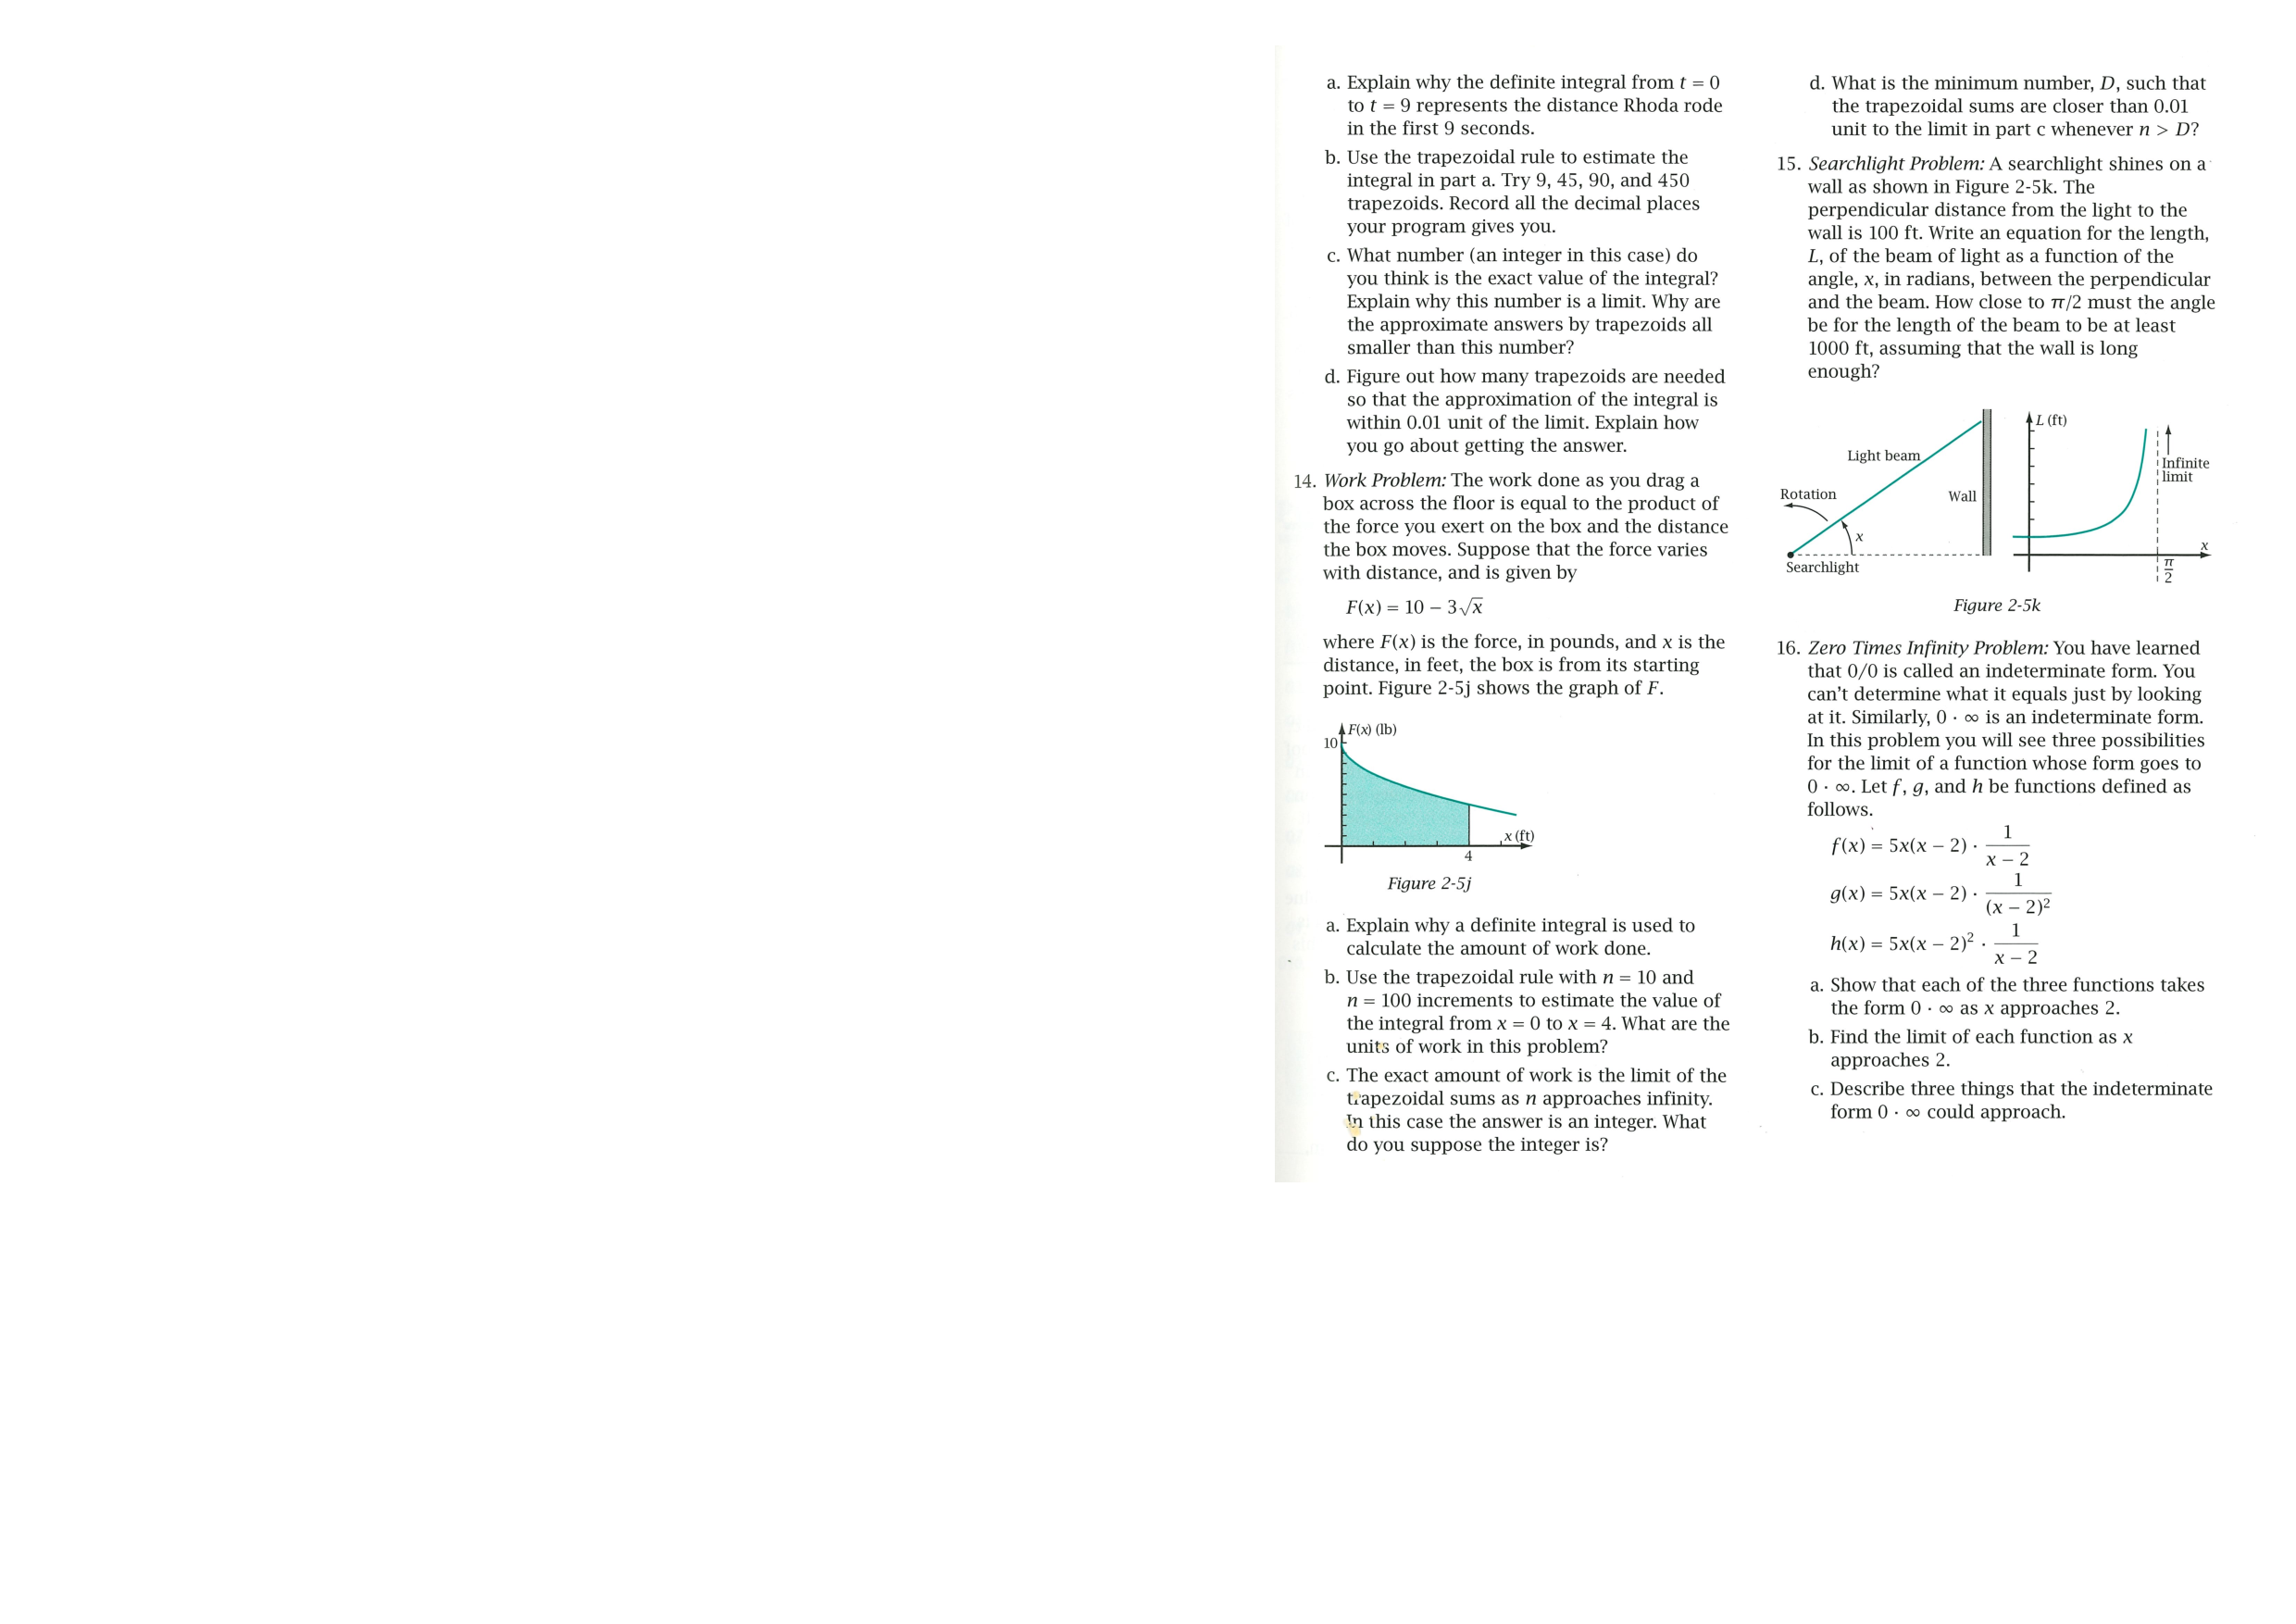
\includegraphics[width=\paperwidth]{\chapdir/0204xC.pdf}}



%									2 - 5
\section{Change}
\subsection{Extremely Average}
Word doc
\newpage
%!TEX root =  ../main.tex

\subsection{Difference Quotient}


\objective{Explain the various forms of the difference quotient and their meaning.}


To all appearances, limits seem to be about incredibly precise --- more precise
than anything in our universe --- or unmeasurably large inputs of functions.
This would seem to offer us nothing useful about the world we actually find ourselves
in.  Such is not the case, however.

If we want to know about the rate of change of a function, we must typically ask 
``over what interval?''  We might suspect that there is a moment on the graph below
($x\approx.25$) where the average rate of change is 0.  How might we prove that?
We would have to travel some further amount in the $x$ direction, which would
produce some change in the $y$ value, because the rate of change is $\frac{\Delta y}
{\Delta x}$.

\begin{figure}
\begin{center}
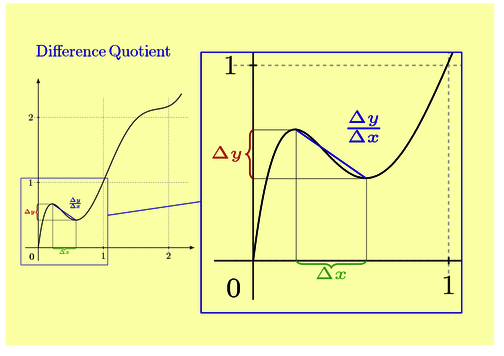
\includegraphics[scale=0.6]{\chapdir/pics/dq.png}
% http://www.texample.net/tikz/examples/difference-quotient/
\caption{The difference quotient, as $\Delta x$ approaches 0\cite{tikzdq}.}
\end{center}
\end{figure}

In single-variable calculus, the difference quotient is usually the name for the expression
\begin{equation}
\lim_{h\rightarrow0}\frac {f(x+h)-f(x)}{(x+h)-x}
\end{equation}

What does this represent?  We are looking for the rate of change of the function.  We begin
by inputting $x$ (and, of course, receiving an output of $f(x)$).  We then move over a tiny 
amount and measure the change in output, over the change in input.  That tiny amount is called
$h$, and we take the limit as $h$ goes to 0.

Because we are evaluating the entire function this way, if we are able to answer the limit, 
we will receive a new function as out answer.  This function is called the \textbf{derivative} of
$f(x)$.


\begin{derivation}{Derivative}
The derivative of a function $f(x)$ may be denoted $f'(x)$.  This style of writing is
called \textbf{Lagrange's notation}, after Joseph-Louis Lagrange
\end{derivation}


\begin{figure}
\begin{center}
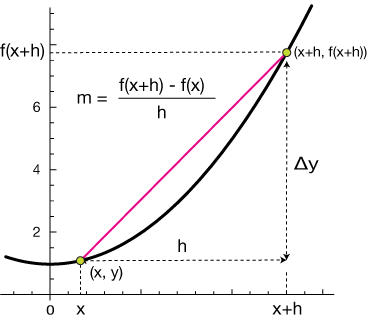
\includegraphics[scale=0.9]{\chapdir/pics/deriv.png}
\caption{The difference quotient produces a secant line \cite{derivativedefinition}.}
\end{center}
\end{figure}

Sometimes it is too difficult or time consuming to find the entire derivative equation.
We might want to find the derivative at one location only, typically called $c$

\begin{equation}
\lim_{x\rightarrow c}\frac{f(x)-f(c)}{x-c}
\end{equation}

These tend to be much easier to solve, as they are typically removable discontinuities
of the kind we solved in §2.1

\subsection{Theorems of Limits}
Let's us generalize the properties of limits we have seen in action this chapter:
\begin{enumerate}
\item The limit of a product is the same as a product of limits
\item The limit of a sum is the same as a sum of limits
\item The limit of a quotient is the same as a quotient of limits (but $\ne 0$)
\item The limit of a constant times a function is the same as a constant times a limit
\item the limit of a constant is a constant
\end{enumerate}

~\vfill
%\newpage
\subsection{Exercises}
\noindent\makebox[\textwidth]{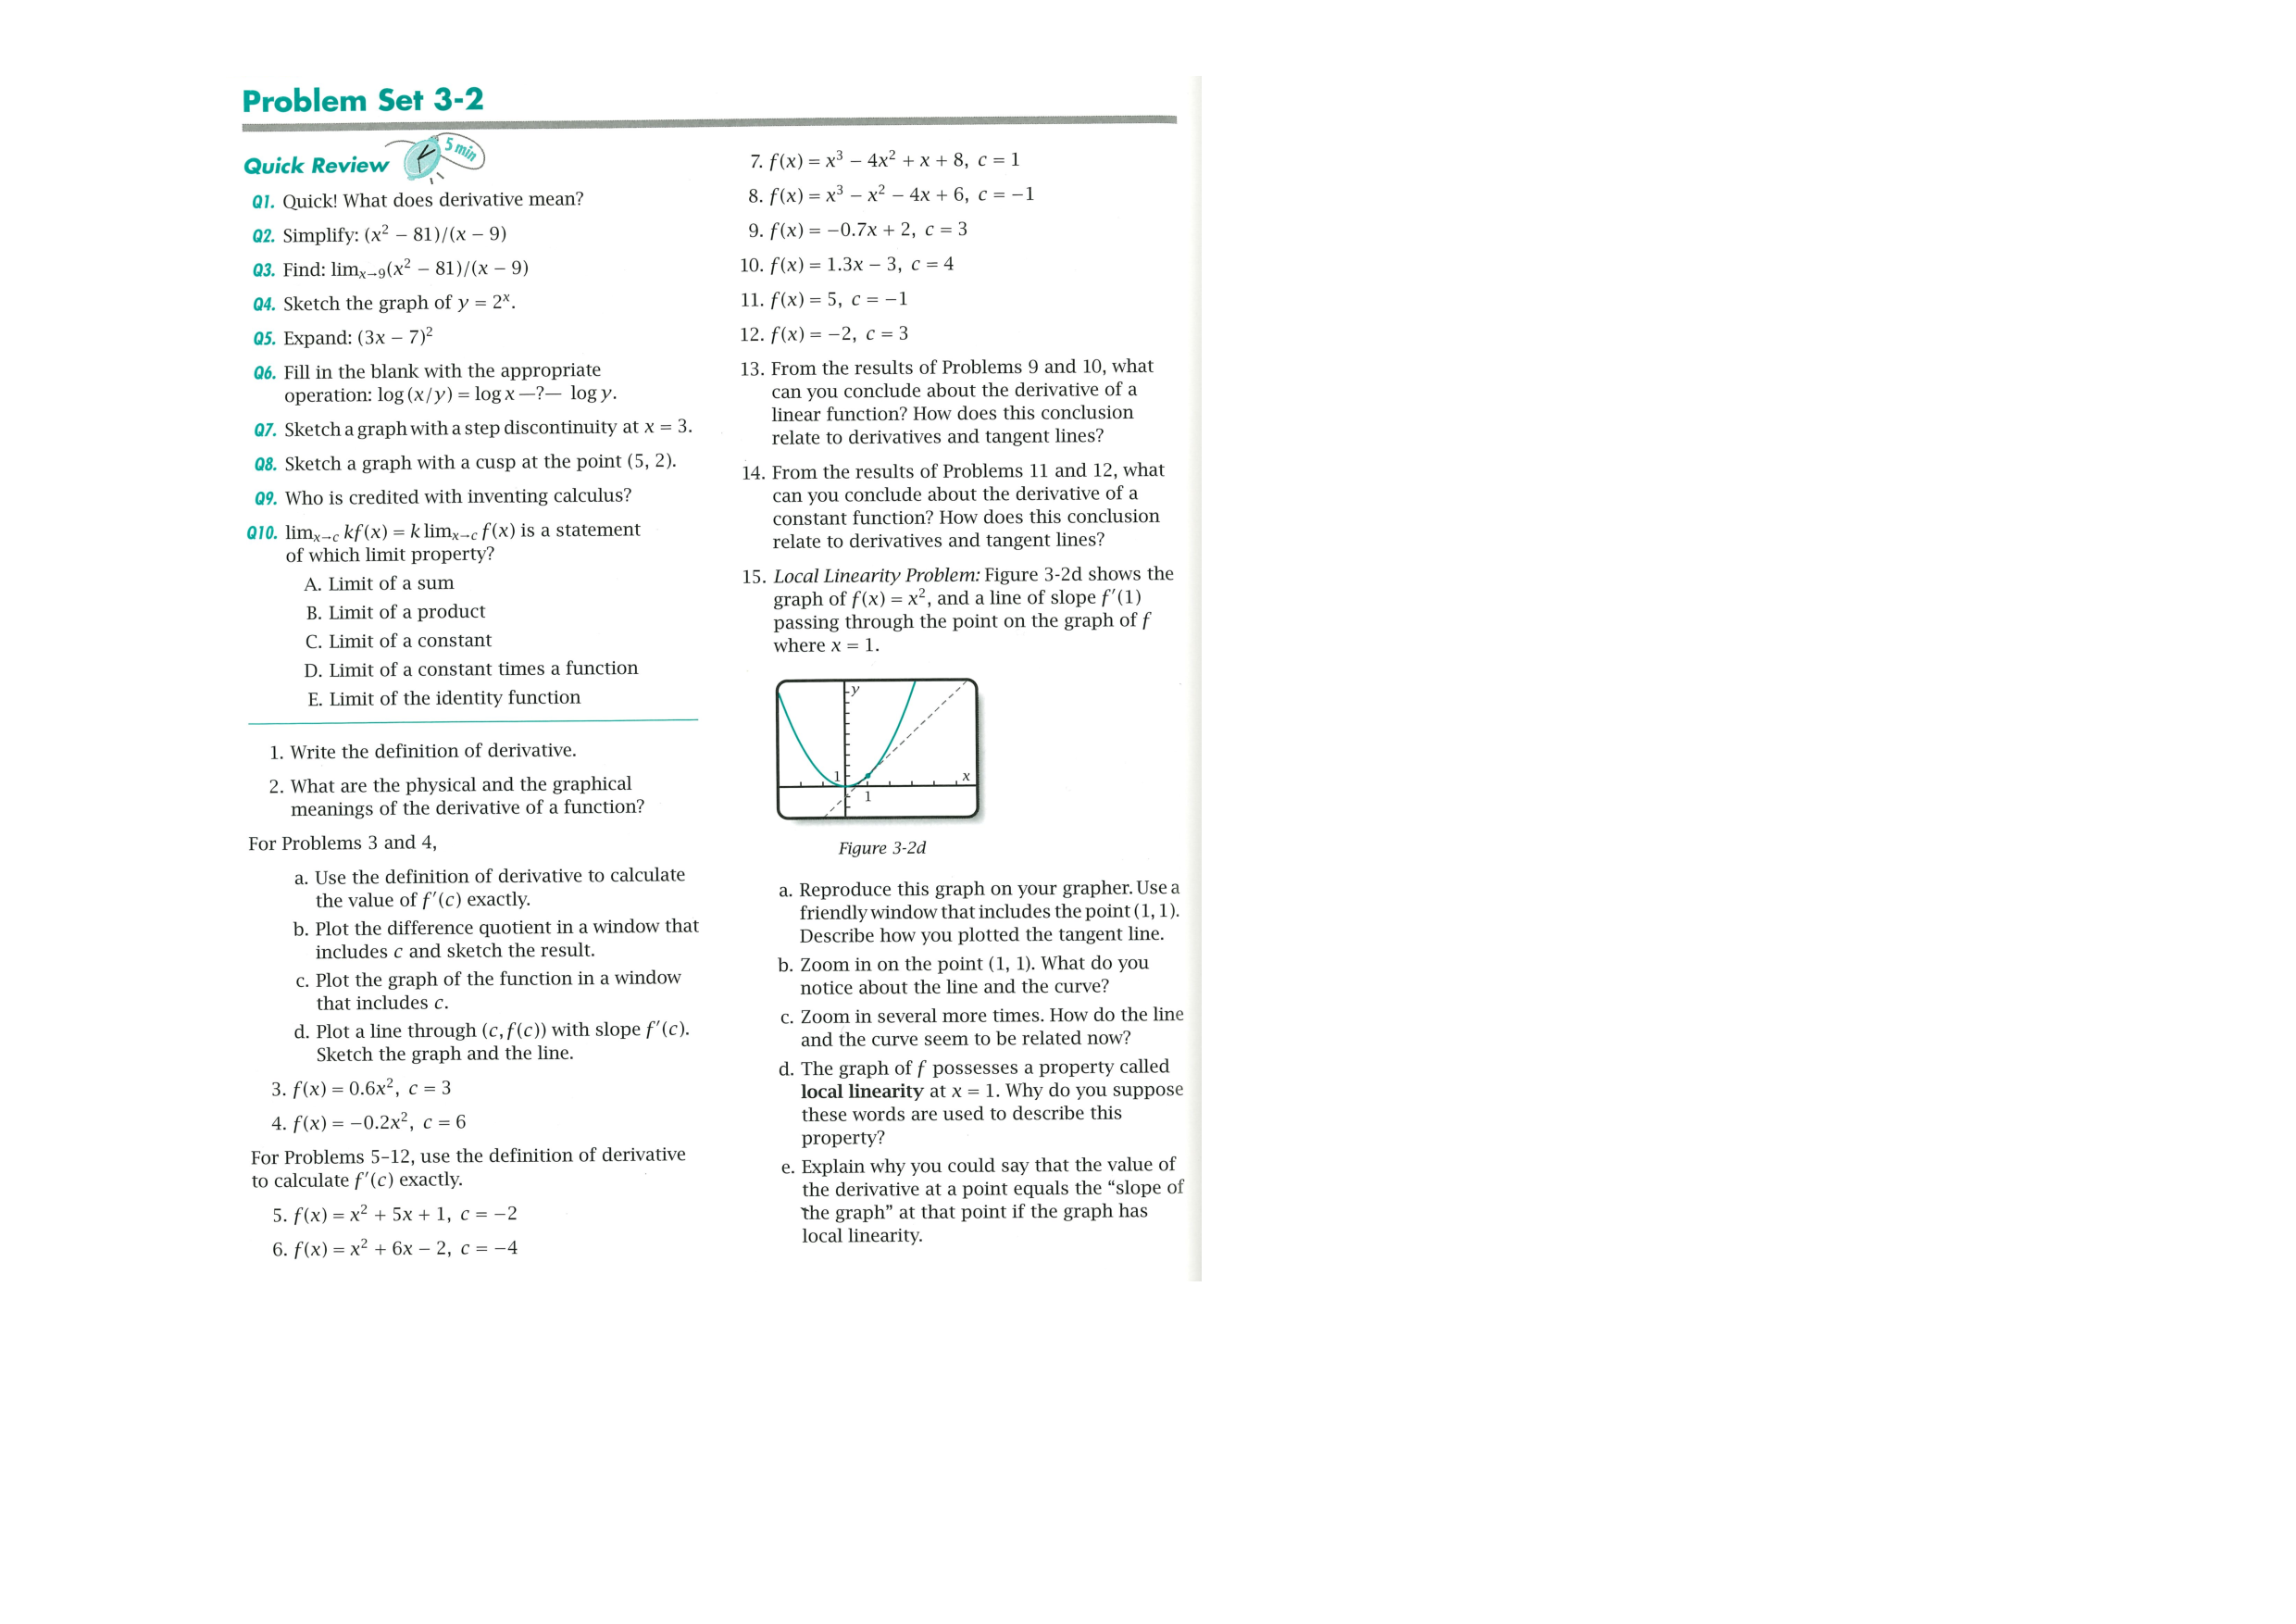
\includegraphics[width=\paperwidth]{\chapdir/0205xA.pdf}}
\newpage
\noindent\makebox[\textwidth]{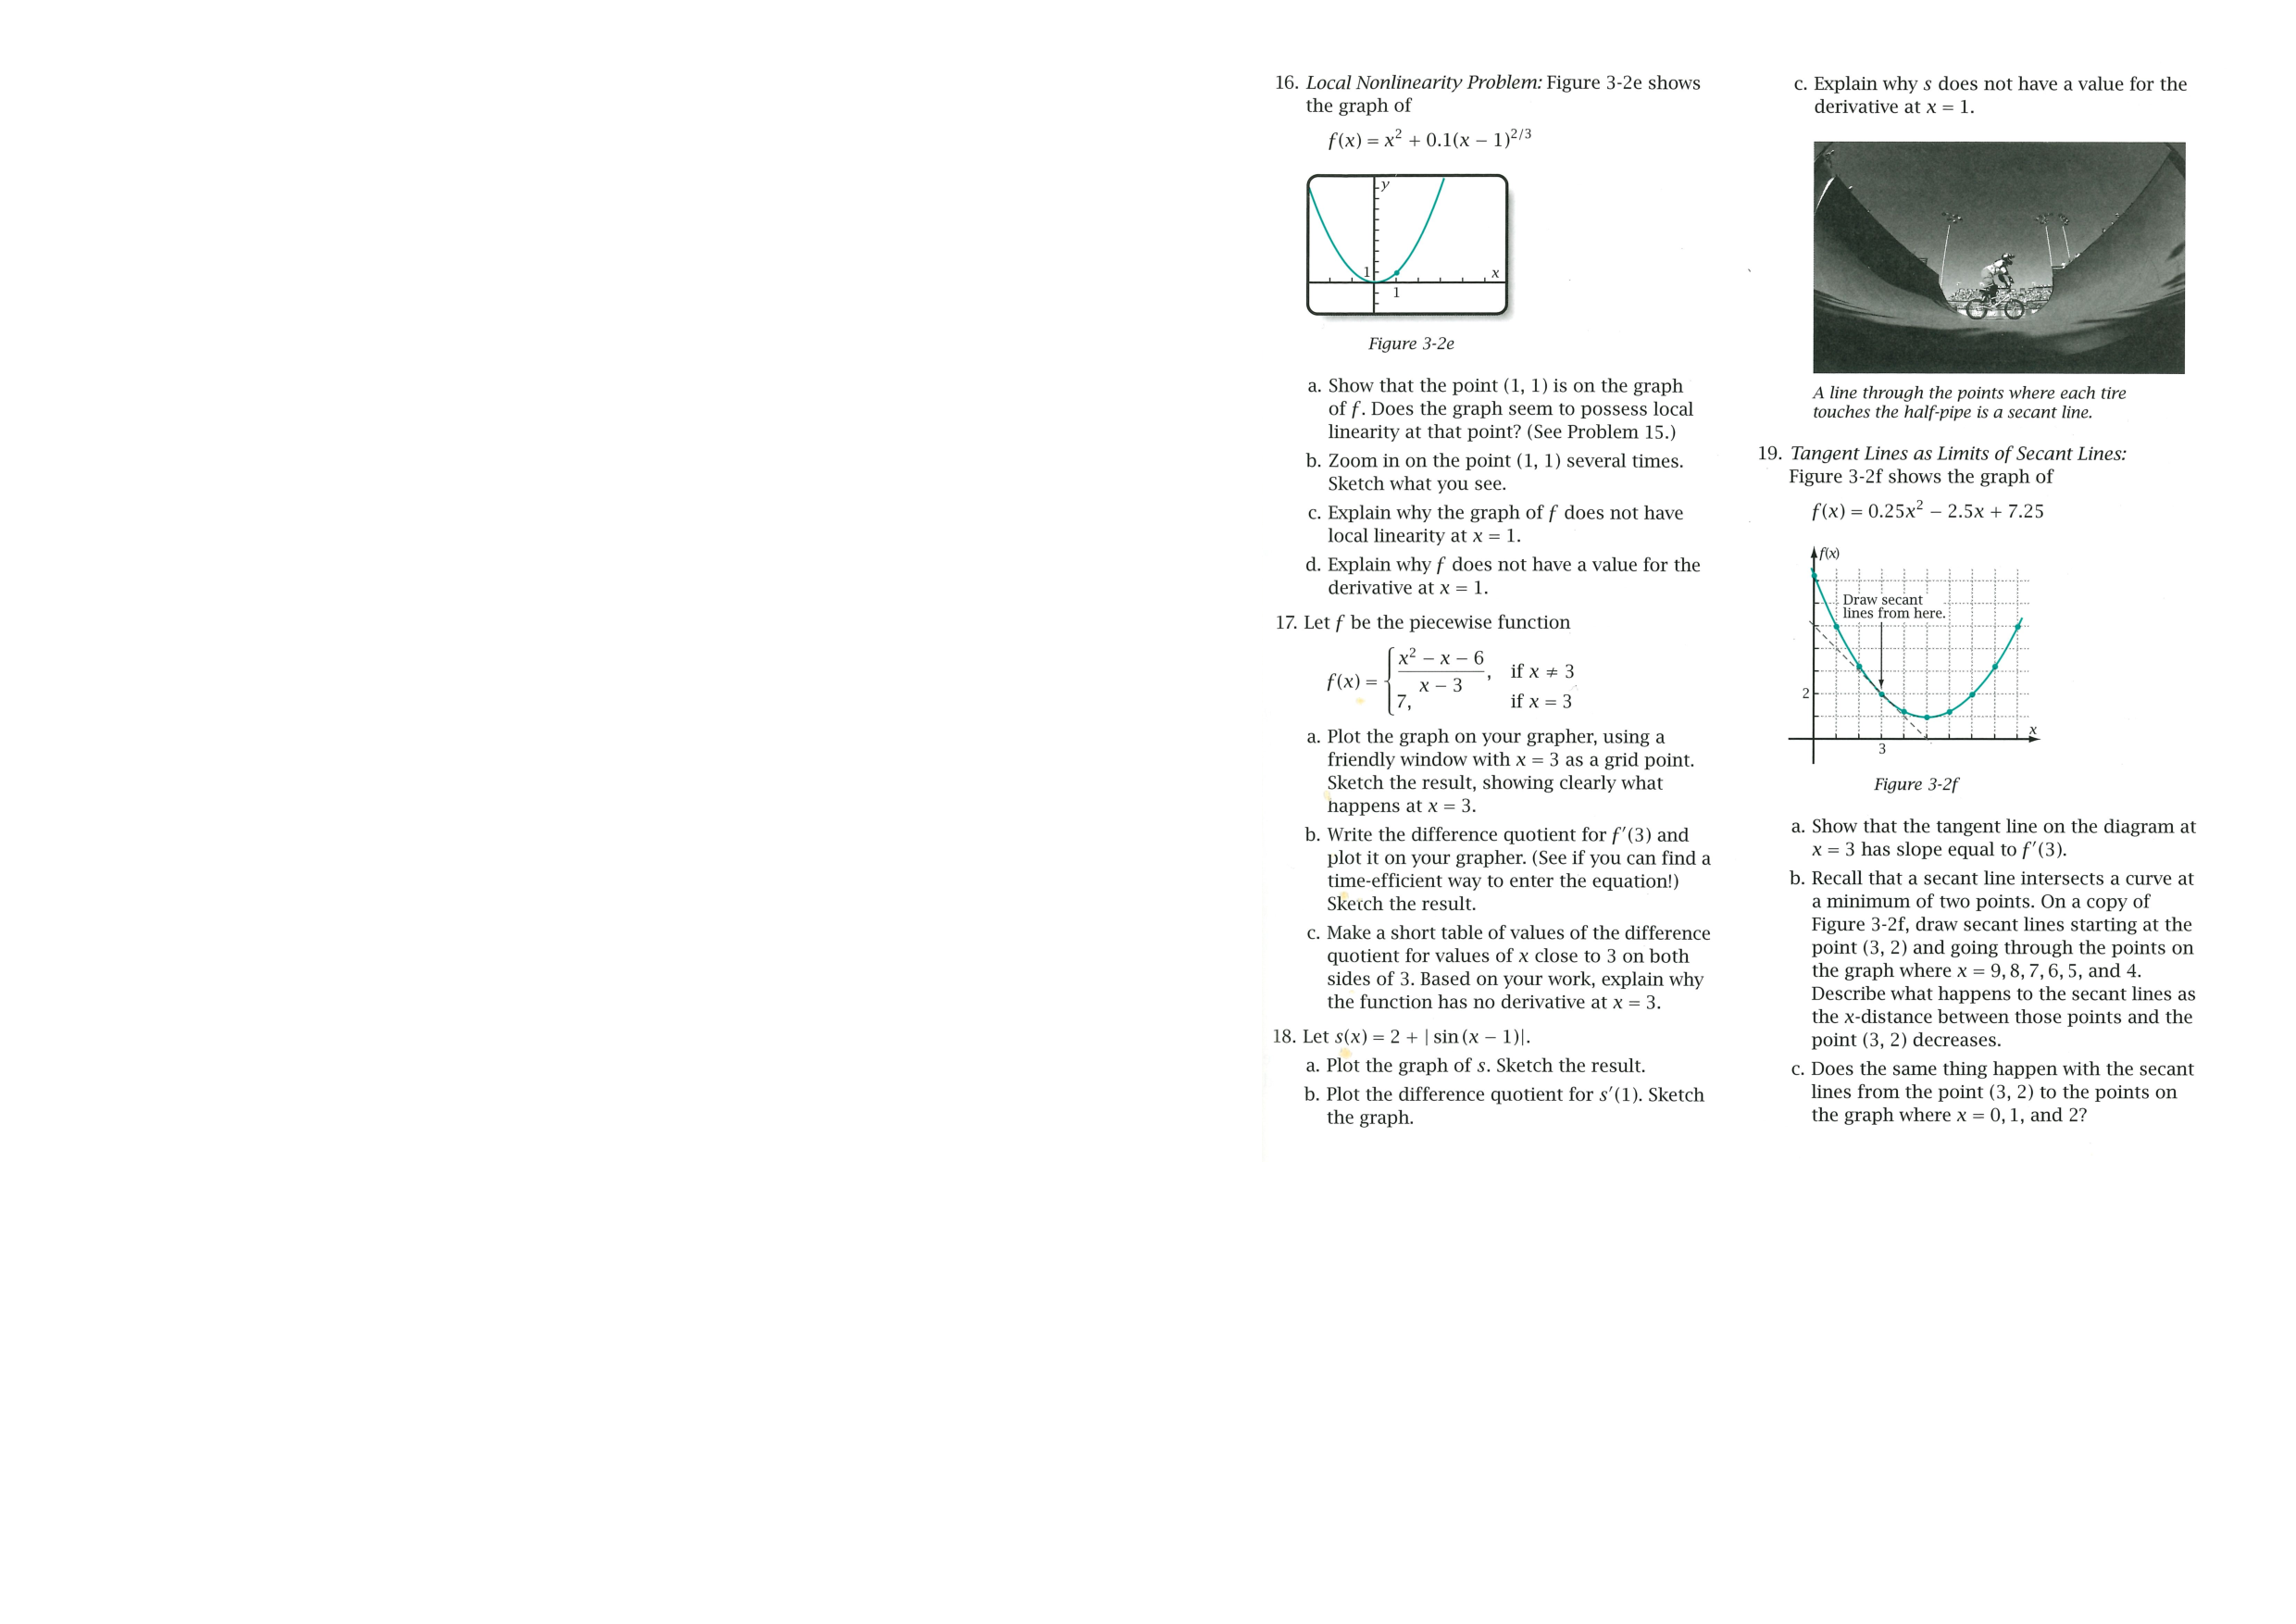
\includegraphics[width=\paperwidth]{\chapdir/0205xB.pdf}}


%									2 - 6
\section{Review}
\subsection{Chapter Review}
This chapter was generally new ideas, that we might describe where a function ``would've gone'',
whether it ended up with a value or not.  This idea --- called a limit --- has a formal definition with
the Greek letters $\epsilon$ and $\delta$, which correspond to the ``error'' in the $y$ values
resulting ``differences'' in the $x$/input.  Limits allowed up to define what a continuous 
function is.  We saw that a function might be composed of pieces ... and still be continuous.
There are four ways to remove discontinuities.  There are five kinds of discontinuities.
The powerful language of limits extended to describe phenomena at infinities, as well as ``values'' 
of the infinities.  Ultimately, limits were used to make possible difference quotients, the 
average rate of change of a function at an instant.

\subsection{Chapter Test}